% Lines starting with a percent sign (%) are comments. LaTeX will 
% not process those lines. Similarly, everything after a percent 
% sign in a line is considered a comment. To produce a percent sign
% in the output, write \% (backslash followed by the percent sign). 
% ==================================================================
% Usage instructions:
% ------------------------------------------------------------------
% The file is heavily commented so that you know what the various
% commands do. Feel free to remove any comments you don't need from
% your own copy. When redistributing the example thesis file, please
% retain all the comments for the benefit of other thesis writers! 
% ==================================================================
% Compilation instructions: 
% ------------------------------------------------------------------
% Use pdflatex to compile! Input images are expected as PDF files.
% Example compilation:
% ------------------------------------------------------------------
% > pdflatex thesis-example.tex
% > bibtex thesis-example
% > pdflatex thesis-example.tex
% > pdflatex thesis-example.tex
% ------------------------------------------------------------------
% You need to run pdflatex multiple times so that all the cross-references
% are fixed. pdflatex will tell you if you need to re-run it (a warning
% will be issued)  
% ------------------------------------------------------------------
% Compilation has been tested to work in ukk.cs.hut.fi and kosh.hut.fi
% - if you have problems of missing .sty -files, then the local LaTeX
% environment does not have all the required packages installed.
% For example, when compiling in vipunen.hut.fi, you get an error that
% tikz.sty is missing - in this case you must either compile somewhere
% else, or you cannot use TikZ graphics in your thesis and must therefore
% remove or comment out the tikz package and all the tikz definitions. 
% ------------------------------------------------------------------

% General information
% ==================================================================
% Package documentation:
% 
% The comments often refer to package documentation. (Almost) all LaTeX
% packages have documentation accompanying them, so you can read the
% package documentation for further information. When a package 'xxx' is
% installed to your local LaTeX environment (the document compiles
% when you have \usepackage{xxx} and LaTeX does not complain), you can 
% find the documentation somewhere in the local LaTeX texmf directory
% hierarchy. In ukk.cs.hut.fi, this is /usr/texlive/2008/texmf-dist,
% and the documentation for the titlesec package (for example) can be 
% found at /usr/texlive/2008/texmf-dist/doc/latex/titlesec/titlesec.pdf.
% Most often the documentation is located as a PDF file in 
% /usr/texlive/2008/texmf-dist/doc/latex/xxx, where xxx is the package name; 
% however, documentation for TikZ is in
% /usr/texlive/2008/texmf-dist/doc/latex/generic/pgf/pgfmanual.pdf
% (this is because TikZ is a front-end for PGF, which is meant to be a 
% generic portable graphics format for LaTeX).
% You can try to look for the package manual using the ``find'' shell
% command in Linux machines; the find databases are up-to-date at least
% in ukk.cs.hut.fi. Just type ``find xxx'', where xxx is the package
% name, and you should find a documentation file.
% Note that in some packages, the documentation is in the DVI file
% format. In this case, you can copy the DVI file to your home directory,
% and convert it to PDF with the dvipdfm command (or you can read the
% DVI file directly with a DVI viewer).
% 
% If you can't find the documentation for a package, just try Googling
% for ``latex packagename''; most often you can get a direct link to the
% package manual in PDF format.
% ------------------------------------------------------------------


% Document class for the thesis is report
% ------------------------------------------------------------------
% You can change this but do so at your own risk - it may break other things.
% Note that the option pdftext is used for pdflatex; there is no
% pdflatex option. 
% ------------------------------------------------------------------
\documentclass[12pt,a4paper,oneside,pdftex]{report}

% The input files (tex files) are encoded with the latin-1 encoding 
% (ISO-8859-1 works). Change the latin1-option if you use UTF8 
% (at some point LaTeX did not work with UTF8, but I'm not sure
% what the current situation is) 
\usepackage[latin1]{inputenc}
% OT1 font encoding seems to work better than T1. Check the rendered
% PDF file to see if the fonts are encoded properly as vectors (instead
% of rendered bitmaps). You can do this by zooming very close to any letter 
% - if the letter is shown pixelated, you should change this setting 
% (try commenting out the entire line, for example).  
\usepackage[OT1]{fontenc}
% The babel package provides hyphenating instructions for LaTeX. Give
% the languages you wish to use in your thesis as options to the babel
% package (as shown below). You can remove any language you are not
% going to use.
% Examples of valid language codes: english (or USenglish), british, 
% finnish, swedish; and so on.
\usepackage[english]{babel}


% Font selection
% ------------------------------------------------------------------
% The default LaTeX font is a very good font for rendering your 
% thesis. It is a very professional font, which will always be 
% accepted. 
% If you, however, wish to spicen up your thesis, you can try out
% these font variants by uncommenting one of the following lines
% (or by finding another font package). The fonts shown here are 
% all fonts that you could use in your thesis (not too silly). 
% Changing the font causes the layouts to shift a bit; you many
% need to manually adjust some layouts. Check the warning messages
% LaTeX gives you.
% ------------------------------------------------------------------
% To find another font, check out the font catalogue from
% http://www.tug.dk/FontCatalogue/mathfonts.html
% This link points to the list of fonts that support maths, but
% that's a fairly important point for master's theses.
% ------------------------------------------------------------------
% <rant>
% Remember, there is no excuse to use Comic Sans, ever, in any
% situation! (Well, maybe in speech bubbles in comics, but there 
% are better options for those too)
% </rant>

% \usepackage{palatino}
% \usepackage{tgpagella}



% Optional packages
% ------------------------------------------------------------------
% Select those packages that you need for your thesis. You may delete
% or comment the rest.

% Natbib allows you to select the format of the bibliography references.
% The first example uses numbered citations: 
\usepackage[square,sort&compress,numbers]{natbib}
% The second example uses author-year citations.
% If you use author-year citations, change the bibliography style (below); 
% acm style does not work with author-year citations.
% Also, you should use \citet (cite in text) when you wish to refer
% to the author directly (\citet{blaablaa} said blaa blaa), and 
% \citep when you wish to refer similarly than with numbered citations
% (It has been said that blaa blaa~\citep{blaablaa}).
% \usepackage[square]{natbib}

% The alltt package provides an all-teletype environment that acts
% like verbatim but you can use LaTeX commands in it. Uncomment if 
% you want to use this environment. 
% \usepackage{alltt}

% The eurosym package provides a euro symbol. Use with \euro{}
\usepackage{eurosym} 

% Verbatim provides a standard teletype environment that renderes
% the text exactly as written in the tex file. Useful for code
% snippets (although you can also use the listings package to get
% automatic code formatting). 
\usepackage{verbatim}

% The listing package provides automatic code formatting utilities
% so that you can copy-paste code examples and have them rendered
% nicely. See the package documentation for details.
% \usepackage{listings}

% The fancuvrb package provides fancier verbatim environments 
% (you can, for example, put borders around the verbatim text area
% and so on). See package for details.
% \usepackage{fancyvrb}

% Supertabular provides a tabular environment that can span multiple 
% pages. 
%\usepackage{supertabular}
% Longtable provides a tabular environment that can span multiple 
% pages. This is used in the example acronyms file. 
\usepackage{longtable}

% The fancyhdr package allows you to set your the page headers 
% manually, and allows you to add separator lines and so on. 
% Check the package documentation. 
% \usepackage{fancyhdr}

% Subfigure package allows you to use subfigures (i.e. many subfigures
% within one figure environment). These can have different labels and
% they are numbered automatically. Check the package documentation. 
\usepackage{subfigure}

% The titlesec package can be used to alter the look of the titles 
% of sections, chapters, and so on. This example uses the ``medium'' 
% package option which sets the titles to a medium size, making them
% a bit smaller than what is the default. You can fine-tune the 
% title fonts and sizes by using the package options. See the package
% documentation.
\usepackage[medium]{titlesec}

% The TikZ package allows you to create professional technical figures.
% The learning curve is quite steep, but it is definitely worth it if 
% you wish to have really good-looking technical figures. 
\usepackage{tikz}
% You also need to specify which TikZ libraries you use
\usetikzlibrary{positioning}
\usetikzlibrary{calc}
\usetikzlibrary{arrows}
\usetikzlibrary{decorations.pathmorphing,decorations.markings}
\usetikzlibrary{shapes}
\usetikzlibrary{patterns}
\newcommand*\circled[1]{\tikz[baseline=(char.base)]{
		\node[shape=circle,draw,inner sep=2pt] (char) {#1};}}

% The aalto-thesis package provides typesetting instructions for the
% standard master's thesis parts (abstracts, front page, and so on)
% Load this package second-to-last, just before the hyperref package.
% Options that you can use: 
%   mydraft - renders the thesis in draft mode. 
%             Do not use for the final version. 
%   doublenumbering - [optional] number the first pages of the thesis
%                     with roman numerals (i, ii, iii, ...); and start
%                     arabic numbering (1, 2, 3, ...) only on the 
%                     first page of the first chapter
%   twoinstructors  - changes the title of instructors to plural form
%   twosupervisors  - changes the title of supervisors to plural form
\usepackage[mydraft,twosupervisors]{aalto-thesis}
%\usepackage[mydraft,doublenumbering]{aalto-thesis}
%\usepackage{aalto-thesis}
\usepackage{todonotes}
\usepackage{array}
\usepackage{caption}
\usepackage{listings}
\captionsetup[table]{font=small,skip=7pt}     %% Adjust here
\captionsetup[figure]{font=small,skip=7pt}     %% Adjust here
\usepackage[font=small,skip=4pt]{caption}
\usepackage{graphicx}
% Hyperref
% ------------------------------------------------------------------
% Hyperref creates links from URLs, for references, and creates a
% TOC in the PDF file.
% This package must be the last one you include, because it has
% compatibility issues with many other packages and it fixes
% those issues when it is loaded.   
\RequirePackage[pdftex]{hyperref}
% Setup hyperref so that links are clickable but do not look 
% different
\hypersetup{colorlinks=false,raiselinks=false,breaklinks=true}
\hypersetup{pdfborder={0 0 0}}
\hypersetup{bookmarksnumbered=true}
% The following line suggests the PDF reader that it should show the 
% first level of bookmarks opened in the hierarchical bookmark view. 
\hypersetup{bookmarksopen=true,bookmarksopenlevel=1}
% Hyperref can also set up the PDF metadata fields. These are
% set a bit later on, after the thesis setup.   


% Thesis setup
% ==================================================================
% Change these to fit your own thesis.
% \COMMAND always refers to the English version;
% \FCOMMAND refers to the Finnish version; and
% \SCOMMAND refers to the Swedish version.
% You may comment/remove those language variants that you do not use
% (but then you must not include the abstracts for that language)
% ------------------------------------------------------------------
% If you do not find the command for a text that is shown in the cover page or
% in the abstract texts, check the aalto-thesis.sty file and locate the text
% from there. 
% All the texts are configured in language-specific blocks (lots of commands
% that look like this: \renewcommand{\ATCITY}{Espoo}.
% You can just fix the texts there. Just remember to check all the language
% variants you use (they are all there in the same place). 
% ------------------------------------------------------------------
\newcommand{\TITLE}{Simulating energy-aware networks in large-scale distributed systems}
\newcommand{\FTITLE}{}
\newcommand{\STITLE}{}
\newcommand{\SUBTITLE}{}
\newcommand{\FSUBTITLE}{}
\newcommand{\SSUBTITLE}{}
\newcommand{\DATE}{June 26, 2017}
\newcommand{\FDATE}{June 26, 2017}
\newcommand{\SDATE}{June 26, 2017}

% Supervisors and instructors
% ------------------------------------------------------------------
% If you have two supervisors, write both names here, separate them with a 
% double-backslash (see below for an example)
% Also remember to add the package option ``twosupervisors'' or
% ``twoinstructors'' to the aalto-thesis package so that the titles are in
% plural.
% Example of one supervisor:
%\newcommand{\SUPERVISOR}{Professor Antti Yl�-J��ski}
%\newcommand{\FSUPERVISOR}{Professori Antti Yl�-J��ski}
%\newcommand{\SSUPERVISOR}{Professor Antti Yl�-J��ski}
% Example of twosupervisors:
\newcommand{\SUPERVISOR}{Professor Martin Quinson\\
  Dr. Anne-C�cile Orgerie}

\newcommand{\FSUPERVISOR}{Professor Martin Quinson\\
	Dr. Anne-C�cile Orgerie}
\newcommand{\SSUPERVISOR}{Professor Martin Quinson\\
	Dr. Anne-C�cile Orgerie}

% If you have only one instructor, just write one name here
\newcommand{\INSTRUCTOR}{Olli Ohjaaja M.Sc. (Tech.)}
\newcommand{\FINSTRUCTOR}{Diplomi-insin��ri Olli Ohjaaja}
\newcommand{\SINSTRUCTOR}{Diplomingenj�r Olli Ohjaaja}
% If you have two instructors, separate them with \\ to create linefeeds
% \newcommand{\INSTRUCTOR}{Olli Ohjaaja M.Sc. (Tech.)\\
%  Elli Opas M.Sc. (Tech)}
%\newcommand{\FINSTRUCTOR}{Diplomi-insin��ri Olli Ohjaaja\\
%  Diplomi-insin��ri Elli Opas}
%\newcommand{\SINSTRUCTOR}{Diplomingenj�r Olli Ohjaaja\\
%  Diplomingenj�r Elli Opas}

% If you have two supervisors, it is common to write the schools
% of the supervisors in the cover page. If the following command is defined,
% then the supervisor names shown here are printed in the cover page. Otherwise,
% the supervisor names defined above are used.
\newcommand{\COVERSUPERVISOR}{Professor Antti Yl�-J��ski, Aalto University\\
  Professor Pekka Perustieteilij�, University of Helsinki}

% The same option is for the instructors, if you have multiple instructors.
% \newcommand{\COVERINSTRUCTOR}{Olli Ohjaaja M.Sc. (Tech.), Aalto University\\
%  Elli Opas M.Sc. (Tech), Aalto SCI}


% Other stuff
% ------------------------------------------------------------------
\newcommand{\PROFESSORSHIP}{Data Communication Software}
\newcommand{\FPROFESSORSHIP}{Tietoliikenneohjelmistot}
\newcommand{\SPROFESSORSHIP}{Datakommunikationsprogram}
% Professorship code is the same in all languages
\newcommand{\PROFCODE}{T-110}
\newcommand{\KEYWORDS}{ocean, sea, marine, ocean mammal, marine mammal, whales,
cetaceans, dolphins, porpoises}
\newcommand{\FKEYWORDS}{AEL, aineistot, aitta, akustiikka, Alankomaat,
aluerakentaminen, Anttolanhovi, Arcada, ArchiCad, arkki}
\newcommand{\SKEYWORDS}{oms�ttning, kassafl�de, v�rdepappersmarknadslagen,
yrkesut�vare, intressef�retag, verifieringskedja}
\newcommand{\LANGUAGE}{English}
\newcommand{\FLANGUAGE}{Englanti}
\newcommand{\SLANGUAGE}{Engelska}

% Author is the same for all languages
\newcommand{\AUTHOR}{Betsegaw Lemma Amersho}


% Currently the English versions are used for the PDF file metadata
% Set the PDF title
\hypersetup{pdftitle={\TITLE\ \SUBTITLE}}
% Set the PDF author
\hypersetup{pdfauthor={\AUTHOR}}
% Set the PDF keywords
\hypersetup{pdfkeywords={\KEYWORDS}}
% Set the PDF subject
\hypersetup{pdfsubject={Master's Thesis}}

\sloppy
% Layout settings
% ------------------------------------------------------------------

% When you write in English, you should use the standard LaTeX 
% paragraph formatting: paragraphs are indented, and there is no 
% space between paragraphs.
% When writing in Finnish, we often use no indentation in the
% beginning of the paragraph, and there is some space between the 
% paragraphs. 

% If you write your thesis Finnish, uncomment these lines; if 
% you write in English, leave these lines commented! 
% \setlength{\parindent}{0pt}
% \setlength{\parskip}{1ex}

% Use this to control how much space there is between each line of text.
% 1 is normal (no extra space), 1.3 is about one-half more space, and
% 1.6 is about double line spacing.  
% \linespread{1} % This is the default
% \linespread{1.3}

% Bibliography style
% acm style gives you a basic reference style. It works only with numbered
% references.
\bibliographystyle{acm}
% Plainnat is a plain style that works with both numbered and name citations.
% \bibliographystyle{plainnat}


% Extra hyphenation settings
% ------------------------------------------------------------------
% You can list here all the files that are not hyphenated correctly.
% You can provide many \hyphenation commands and/or separate each word
% with a space inside a single command. Put hyphens in the places where
% a word can be hyphenated.
% Note that (by default) LaTeX will not hyphenate words that already
% have a hyphen in them (for example, if you write ``structure-modification 
% operation'', the word structure-modification will never be hyphenated).
% You need a special package to hyphenate those words.
\hyphenation{di-gi-taa-li-sta yksi-suun-tai-sta}



% The preamble ends here, and the document begins. 
% Place all formatting commands and such before this line.
% ------------------------------------------------------------------
\begin{document}
% This command adds a PDF bookmark to the cover page. You may leave
% it out if you don't like it...
\pdfbookmark[0]{Cover page}{bookmark.0.cover}
% This command is defined in aalto-thesis.sty. It controls the page 
% numbering based on whether the doublenumbering option is specified
\startcoverpage

% Cover page
% ------------------------------------------------------------------
% Options: finnish, english, and swedish
% These control in which language the cover-page information is shown
\coverpage{english}


% Abstracts
% ------------------------------------------------------------------
% Include an abstract in the language that the thesis is written in,
% and if your native language is Finnish or Swedish, one in that language.

% Abstract in English
% ------------------------------------------------------------------
\thesisabstract{english}{
A dissertation or thesis is a document submitted in support of candidature
for a degree or professional qualification presenting the author's research and
findings. In some countries/universities, the word thesis or a cognate is used
as part of a bachelor's or master's course, while dissertation is normally
applied to a doctorate, whilst, in others, the reverse is true.

\fixme{Abstract text goes here (and this is an example how to use fixme).} 
Fixme is a command that helps you identify parts of your thesis that still
require some work. When compiled in the custom \texttt{mydraft} mode, text
parts tagged with fixmes are shown in bold and with fixme tags around them. When
compiled in normal mode, the fixme-tagged text is shown normally (without
special formatting). The draft mode also causes the ``Draft'' text to appear on
the front page, alongside with the document compilation date. The custom
\texttt{mydraft} mode is selected by the \texttt{mydraft} option given for the
package \texttt{aalto-thesis}, near the top of the \texttt{thesis-example.tex}
file.

The thesis example file (\texttt{thesis-example.tex}), all the chapter content
files (\texttt{1introduction.tex} and so on), and the Aalto style file
(\texttt{aalto-thesis.sty}) are commented with explanations on how the Aalto
thesis works. The files also contain some examples on how to customize various
details of the thesis layout, and of course the example text works as an
example in itself. Please read the comments and the example text; that should
get you well on your way!}


% Acknowledgements
% ------------------------------------------------------------------
% Select the language you use in your acknowledgements
\selectlanguage{english}

% Uncomment this line if you wish acknoledgements to appear in the 
% table of contents
%\addcontentsline{toc}{chapter}{Acknowledgements}

% The star means that the chapter isn't numbered and does not 
% show up in the TOC
\chapter*{Acknowledgements}

I wish to thank all students who use \LaTeX\ for formatting their theses,
because theses formatted with \LaTeX\ are just so nice.

Thank you, and keep up the good work!
\vskip 10mm

\noindent Espoo, \DATE
\vskip 5mm
\noindent\AUTHOR

% Acronyms
% ------------------------------------------------------------------
% Use \cleardoublepage so that IF two-sided printing is used 
% (which is not often for masters theses), then the pages will still
% start correctly on the right-hand side.
\cleardoublepage
% Example acronyms are placed in a separate file, acronyms.tex
\addcontentsline{toc}{chapter}{Abbreviations and Acronyms}
\chapter*{Abbreviations and Acronyms}

% The longtable environment should break the table properly to multiple pages, 
% if needed

\noindent
\begin{longtable}{@{}p{0.25\textwidth}p{0.7\textwidth}@{}}
2k/4k/8k mode & COFDM operation modes \\
3GPP & 3rd Generation Partnership Project \\ 
ESP & Encapsulating Security Payload; An IPsec security protocol \\ 
FLUTE  & The File Delivery over Unidirectional Transport protocol \\ 
e.g.& for example (do not list here this kind of common acronymbs or abbreviations, but only those that are essential for understanding the content of your thesis. \\ 
note & Note also, that this list is not compulsory, and should be omitted if you have only few abbreviations

\end{longtable}


% Table of contents
% ------------------------------------------------------------------
\cleardoublepage
% This command adds a PDF bookmark that links to the contents.
% You can use \addcontentsline{} as well, but that also adds contents
% entry to the table of contents, which is kind of redundant.
% The text ``Contents'' is shown in the PDF bookmark. 
\pdfbookmark[0]{Contents}{bookmark.0.contents}
\tableofcontents

% List of tables
% ------------------------------------------------------------------
% You only need a list of tables for your thesis if you have very 
% many tables. If you do, uncomment the following two lines.
% \cleardoublepage
% \listoftables

% Table of figures
% ------------------------------------------------------------------
% You only need a list of figures for your thesis if you have very 
% many figures. If you do, uncomment the following two lines.
% \cleardoublepage
% \listoffigures

% The following label is used for counting the prelude pages
\label{pages-prelude}
\cleardoublepage

%%%%%%%%%%%%%%%%% The main content starts here %%%%%%%%%%%%%%%%%%%%%
% ------------------------------------------------------------------
% This command is defined in aalto-thesis.sty. It controls the page 
% numbering based on whether the doublenumbering option is specified
\startfirstchapter

% Add headings to pages (the chapter title is shown)
\pagestyle{headings}

% The contents of the thesis are separated to their own files.
% Edit the content in these files, rename them as necessary.
% ------------------------------------------------------------------
\chapter{Introduction}
\label{chapter:intro}
According to the report released from Cisco, "The Zettabyte Era", the number of networked device is expected to increase from 17.1 billion in 2016 to 27.1 billion in 2021. In another report titled "Cisco Global Cloud Index, 2015 to 2020", global cloud IP traffic will grow more than three times and, among all the workloads performed in data-centers, by the year 2020, 92\% of them will be performed in cloud data-centers. The remaining 8\% will be performed in traditional data-centers. In response to this growing trends, the data-centers are continuously expanding. This expansion raises a primary concern on the amount of energy required to support the added data-center components and the growing service demands. 

The energy consumption issue is further aggravated due to the fact that current servers and network devices are energy inefficient. Of the total power consumed by a given computing or communication device, the idle power consumption takes the greater proportion. An IT equipment is considered energy efficient when it consumes power proportional to the amount of computing or data transfer task it performs. Currently there are different techniques implemented at a device level to tackle the energy inefficiency problem. For computing device, for instance, the operating frequency of the CPU can be lowered when the amount of task reach below some threshold value. Similarly, for a communicating devices, the data transferring rate can be lowered (a.k.a, adaptive link rate mode) depending on the traffic or the device can be set to sleep (a.k.a, low power mode) when there is no traffic. However, these techniques are not fully utilized, as the techniques induce performance penalty when switch from one mode to another.  

Solving the energy consumption issue is primarily driven by economical factor, to save energy consumption bills, and environmental factor,to reduce \($$CO_2$$\) emission. There are also other secondary factors, such as reducing the heat generated by a given IT device. The more energy inefficient a device is the more heat it generates. This will intern affect the life time and proper functioning of the device. 

Currently researchers are tackling the energy consumption issue at different levels. At device level, for instance, to find a new  energy saving technique or to optimize the existing ones. At infrastructure level, it can range from finding energy aware routing algorithm for network devices to energy efficient load balancing and workload assignment of servers. 

There are three approaches that are commonly in use for doing energy related research at the infrastructure level. The first approach is to experiments on a real network. Though in this approach one might get the most real picture of the situation at a given moment, it will be very difficult to repeat the experiment on real network due to the transient nature of the experimental parameters such as workload and network traffic.  Furthermore, the real network might not be available for experimentation. The second approach is to use an experimental test-bed. This approach gives full control over the experiment parameters and it is also available. However, when the platform under investigation becomes very large, it will be infeasible to set-up a test-bed for it due to the hardware cost involved. In addition, experimenting on a new hypothesis might require setting up a new test-bed with a new hardware and different configuration. This also become costly and time consuming. The third approach is to use simulation software for experimentation. This approach gives the ultimate control, flexibility and scalability compared to the other two. The main challenge though is accurately modeling the real characteristics of the components involved in the problem at hand.

In the context of computer networking, we can classify simulators into two: packet-level and flow-level simulators. Packet-level simulators strive to capture fine-grain details of a given network. Flow-level simulators, on the other hand, use analytical equations that approximate the behavior of the phenomenon being modeled using few parameters. Compared to flow-level simulators, packet-level simulators are considered more accurate due to the detailed information they try to capture. However, they fail to scale well due to the time and storage they need to process and store the captured information. A typical example of packet-level simulator is NS-3, and of flow-level simulator is SimGrid, a large-scale distributed network simulator. 

Despite the advantages network simulators can offer for studying the energy consumption problem that exist in large-scale networks, search of the literature revealed only few packet-level simulators proposed to address the issue. As we have mentioned earlier, packet-level simulators can not scale well in the area of large-scale networks. Currently, to our knowledge, there is no flow-level simulator proposed that can simulate the energy consumption of computing and communication components of large-scale networks. 

Therefore, the purpose of this study is to investigate the level of accuracy and scalability of flow-level energy consumption simulators for estimating energy consumption of large-scale networks. To fulfill this purpose we use SimGrid simulator. SimGrid already have energy consumption model for computing components, our work is limited to adding flow-level simulation model for communicating devices such as switches and routers. Further more, we are only concerned with wired network components and concepts. 

Our contribution in this work is three-fold. First the proposed flow-level simulator can be used by researchers to find solutions to the energy consumption problem. Second it can also be used by other parties to the mere purpose of estimating energy consumption of large-scale networks. Third, researchers who are interested to do similar work, for instance, in the wireless network, they can follow the method that we outlined in this work.  

The rest of this thesis is organized as follow. In Chapter~\ref{chapter:background}, we first describe relevant concepts that are related to our study and then we review other proposed simulators. In Chapter~\ref{chapter:environment}, we explain about our experimental environment. Then in Chapter~\ref{chapter:methods}, we compare the advantages and disadvantages of commonly used methods that are used to study the energy consumption problem and then we outline the method that we followed. In Chapter~\ref{chapter:implementation} we present the implementation of our flow-level model and then in Chapter~\ref{chapter:evaluation} we discuss about the (in)validation experiment we conducted to evaluate the implementation. Following the validation, in Chapter~\ref{chapter:discussion}, we analyze and discuss the produced result. Finally, in Chapter~\ref{chapter:conclusions} we give concluding remarks and we also forward continuing works that interested researchers might want to follow.




\chapter{Background}
\label{chapter:background} 
In this chapter ...
\section{Electricity consumption of ICT equipments}
\label{section:ictequipment} 
ICT equipments consume a significant amount of electricity. A survey conducted by Heddeghem et al.{\ }\cite{DBLP:journals/comcom/HeddeghemLLCPD14} shows the electricity consumption and growth trends of three classes of ICT equipments: personal computers, communication networks, and data centers. Personal computers include equipments such as desktop, laptop and external monitors. Communication networks includes residential network access equipments (such as WiFi routers and modems), network equipments used in offices (such as routers and switches) and telecom-operator network equipments (such as base stations, routers and optical amplification systems). Data-centers house storage and computing servers, communication network equipments, and power provisioning and cooling facilities.  In this classification there are overlaps, for instance, telcom operator can have office network equipments and data-centers. After carefully avoiding possible redundant measurements, the researchers estimated absolute electricity consumption and annual consumption growth rate of each category of equipments for the period 2007 and 2012. The results of the study show that the global electricity consumption of ICT equipments in all the three categories combined contributed 3.9\% in 2007 and 4.6\% in 2012. The estimated annual growth rate of the individual category is 5\% for personal computers, 10\% for communication networks, and 4\% for data-centers. These growth rates are higher than that of the total global electricity consumption, which is 3\%. 

\section {Data-center electricity consumption}
\label{section:datacenter} 
In Section~\ref{section:ictequipment} we described data-center's global share in electricity consumption. In this section we describe the components involved within the data center itself.

Electricity consumption units with in a typical data-center can be classified into two broad groups \cite{DBLP:journals/comsur/DayarathnaWF16}: The first group is IT equipments (which includes computing servers, storage servers and networking components) and the other group is infrastructure facilities (which includes power provisioning, cooling and lighting components).

Figure~\ref{fig:datacenterenergy} \cite{DBLP:journals/comsur/DayarathnaWF16} shows the electricity consumption proportion of the data-center components. This value differs significantly from one data-center to another \cite{DBLP:series/synthesis/2013Barroso}, for instance, due to architectural difference\cite{DBLP:conf/eenergy/GyarmatiT10} or energy efficiency of the components. The infrastructure facility components take the large proportion (65\%) of the consumption. 
\begin{figure}[ht]
	\begin{center}
		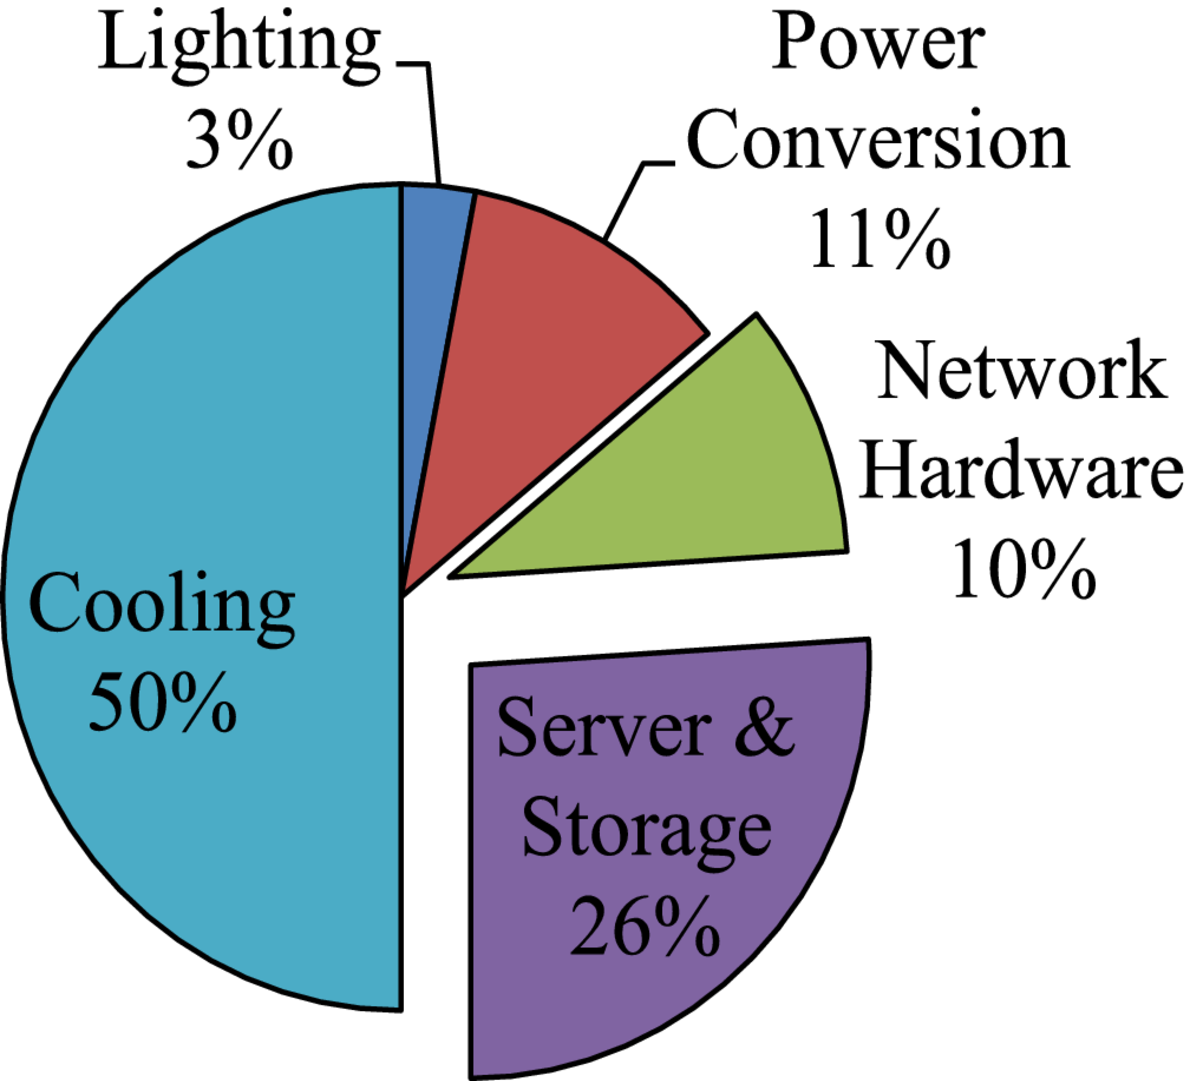
\includegraphics[width=7cm]{images/datacenterenergy.pdf}
		\caption{Energy consumption percentage of data-center components \cite{DBLP:journals/comsur/DayarathnaWF16}}
		\label{fig:datacenterenergy}
	\end{center}
\end{figure}
Though the infrastructure facility consumes relatively larger amount of electricity, the focus of this study is on the IT equipment components, particularly on the network equipments. 

If we further zoom in on the IT equipments part, we can find server, storage and network equipments. A data-center servers consist of one or more CPU cores, memory and I/O devices. The energy consumption relationship among these components is shown in Figure~\ref{fig:serverenergy}. Combined, Memory and CPU units consume the larger amount of energy relative to other components. The fact that CPU is the dominant electricity consuming unit is exploited by Fan et al. in \cite{DBLP:conf/isca/FanWB07} to model the dynamic power usage of thousands of servers by using only CPU utilization as a parameter. The result of their study was very accurate, with error as low as 1\%. 
\begin{figure}[ht]
	\begin{center}
		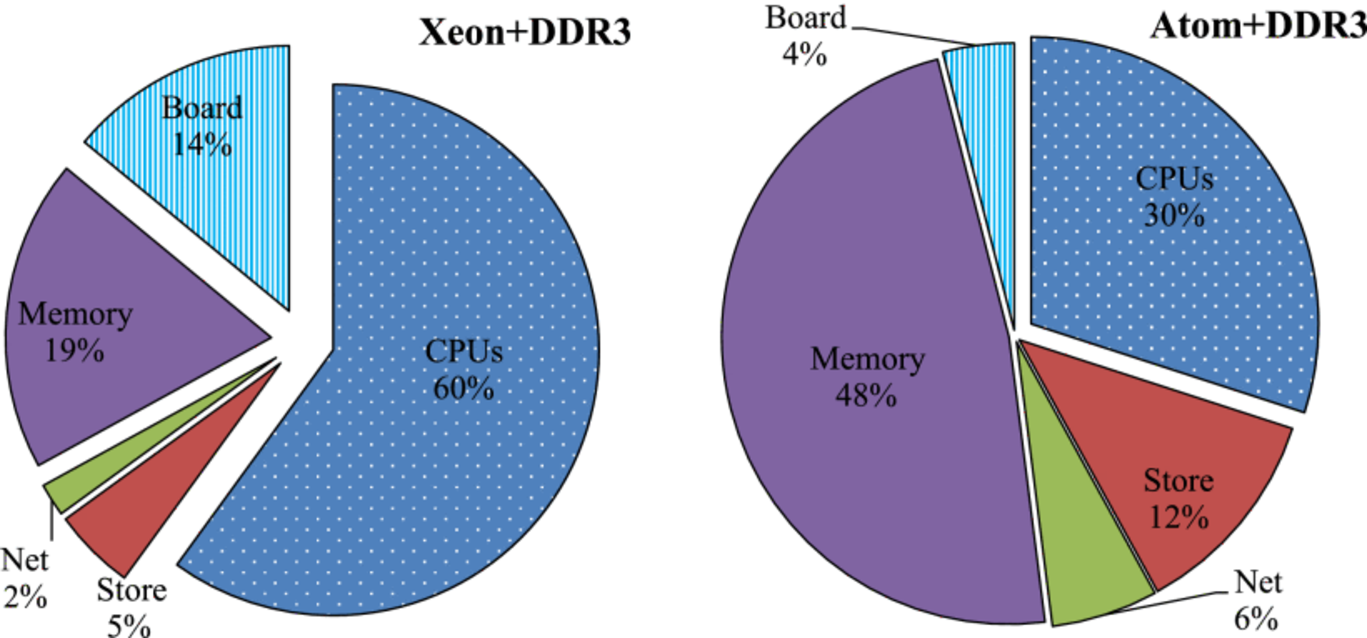
\includegraphics[width=11cm]{images/serverenergy.pdf}
		\caption{Energy consumption percentage of Xeon based (on the left) and Atom based (on the right) servers \cite{DBLP:journals/comsur/DayarathnaWF16}}
		\label{fig:serverenergy}
	\end{center}
\end{figure}
\section{Energy proportionality}
\label{section:energyproportionality}
The primary reason the study of energy consumption management of network equipment becomes so important is that, in general, ICT equipments do not consume energy proportional to their workload. An ideal ICT equipment is the one which consume zero electricity when it is idle, and it consumes electricity proportional to its workload when it is active. However, the reality is, even power efficient servers consume about 50\% of their peak power \cite{DBLP:journals/computer/BarrosoH07}, even when they are doing nothing. This percentage can even reach 85\% for network switches \cite{DBLP:conf/IEEEcloud/FiandrinoKBZ15}. Figure~\ref{fig:energyproportionality} in \cite{DBLP:conf/networking/MahadevanSBR09} shows the energy proportionality of a typical network equipment. From the graph we can observe that the dynamic power consumption range is narrow.
\begin{figure}[ht]
	\begin{center}
		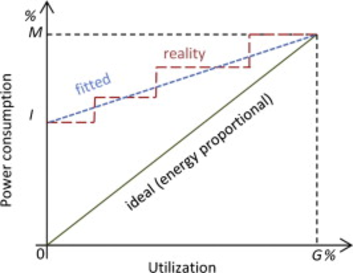
\includegraphics[width=11cm]{images/energyproportionality.pdf}
		\caption{Ideal and measured energy proportionality of a network equipment \cite{DBLP:conf/networking/MahadevanSBR09}}
		\label{fig:energyproportionality}
	\end{center}
\end{figure}
Three approaches are in common use to deal with this situation. The first one is re-engineering network devices so as to make them more energy proportional, device vendors are the prime role player in this aspect. The second approach is related to the operating rate of a network equipment port. A typical switch can operate on different transmission rate (100Mbps, 1 Gbps or 10 Gbps). An active port transmitting at 10 Gbps can consume more energy than if it transmit at 100 Mbps. Rate adaptation is the approach devised to take advantage of this situation. Instead of transmitting at the maximum rate all time,  the network port can be made to adapt to the actual traffic load. This energy saving approach is known as Adaptive Link Rate (ALR). The third approach, which is known as Low Power Idle (LPI), allows a network device to send data as fast as possible and then enter low power mode between transfers. The low power mode can further be extended by a technique called packet coalescing, which allows more energy saving \cite{DBLP:journals/comsur/BollaBDC11}. 
\section{Packet-level and flow-level Simulators}
\label{section:packetflow} 
Packet-level simulators strives to model a given network phenomenon at the granularity level of packets, thus in general they are accepted by the research community to be more accurate compared to flow-level simulators \cite{DBLP:journals/jpdc/CasanovaGLQS14}. One of the most popular packet-level simulator is NS-3, which is categorized under discrete-event simulator with events corresponding to sending and receiving of packets \cite{ns3}. Though packet-level simulators are accepted to be more accurate, they fail to scale well in the area of large-scale networks. 

In the area of large-scale networks, flow-level simulators are the preferred alternative. Rather than modeling a given network phenomenon at a packet level, flow-level simulators treat a set of packets as a single unit \cite{DBLP:journals/jpdc/CasanovaGLQS14}. The most commonly used definition for flow in the context of computer networking is coined by Claffy et al.{\ }in \cite{claffy1998nature}: 

``\ldots a flow \ldots a unidirectional traffic stream with a unique [source-IP-address, source-port, destination-IP-address, destination-port, IP-protocol] tuple \ldots''

In addition to the five tuple mentioned in the definition, a flow also has a limited time duration. Claffy et al.{\ }used a time limit of 64 seconds as a flow duration in their study. Researchers such as Carneiro et al.{\ }\cite{DBLP:conf/valuetools/CarneiroFR09}, adopted this same definition to develop flow monitoring module for NS-3, a module that can generate information such as amount of packets or bytes transferred, packets dropped or transmission start and end time for each flow. Barakat et al. in \cite{DBLP:journals/tsp/BarakatTIDO03} also used the same definition to model traffic at the flow-level for the Internet backbone link. By abstracting away fine details, flow-level models provides easy way to instantiate experiments and they also scale very well for conducting large-scale network simulations \cite{DBLP:journals/jpdc/CasanovaGLQS14,DBLP:journals/tsp/BarakatTIDO03}.

The flow definition given above is not the only one. Any analytical model which capture the characteristics of a given network phenomenon can be considered as flow-level model. In SimGrid, for instance, TCP flow is modeled characterized by bandwidth and end-to-end latency\cite{DBLP:journals/jpdc/CasanovaGLQS14}.
\section{Simulating and modeling energy consumption of large-scale networks}
One way of conducting energy consumption or any other experiment is to use real production environment or test-bed environment, both are referred to as \emph{in vivo} in \cite{DBLP:journals/jpdc/CasanovaGLQS14}. In the former case, handling transient and varying conditions would make the data collection and prediction very difficult and often times, a production environment is not available for experimentation. In the later case, it requires setting-up a separate testing environment designed solely for the purpose of conducting the desired experiment. This approach apart from being expensive, it requires significant amount of time for experiment setup and, it is also non-repeatable as experimenting with different scenario demands a modified or new configuration.

The other alternative for experimenting is simulation, also referred to as \emph{in silico} in \cite{DBLP:journals/jpdc/CasanovaGLQS14}. Simulation, unlike real environment, allows great flexibility in terms of experiment configuration, control and repetition. In addition it can also be less time consuming and less expensive.That is why virtually in all computer network related researches simulations are widely used. 

In this study we simulate energy-aware large scale distributed networks using SimGrid (Detail description about SimGrid follows in the next section). When we say large-scale distributed network, we are referring to a set of networks residing inside in the distributed data centers and also the networks that are used to connect them. 

The energy consumption E of an equipment depends on the operating power P at time t. The total energy consumption for a time period T is given by Equation~\ref{eq:2.1} \cite{DBLP:conf/wowmom/OrgerieLLL11}. 
\begin{equation} \label{eq:2.1}
  E(T) = \int_{0}^{T} P(t) dt
\end{equation} 
Due to the energy proportionality characteristic described in Section~\ref{section:energyproportionality}, the common approach used to compute the energy consumption is to divide the power component into two parts: static/idle power (\($$P_{static}$$\)) and dynamic power (\($$P_{dynamic}$$\)) as shown in equation~\ref{eq:2.2}. Then the total energy is obtained by multiplying the total power, \($$P_{total}$$\) by the time duration \cite{DBLP:conf/wowmom/OrgerieLLL11,DBLP:journals/tjs/KliazovichBK12,DBLP:conf/networking/MahadevanSBR09,DBLP:journals/comsur/DayarathnaWF16}. 
\begin{equation} \label{eq:2.2}
 P_{total} = P_{static} + P_{dynamic}
\end{equation} 
For a typical network equipment such as a switch, the static part constitutes the power consumption of the chassis and the line-cards (when all the ports on the line-cards are switched off). The dynamic part, on the other hand, constitutes the power consumption of the switch ports running at a given rate multiplied by the utilization factor \cite{DBLP:conf/networking/MahadevanSBR09}. Equation~\ref{eq:2.3} shows how to compute the total power for a switch, where \($$P_{switch}$$\), is the total power consumption of a switch, \($$P_{chassis}$$\) and \($$P_{linecard}$$\) is the power consumption of the chassis and the line card, respectively. \($$P_{rate}$$\), is the power consumption of a given port at a given rate and \($$numports_{rate}$$\) is the number of ports running at a given rate. The rate can take values such as 10 Mbps, 100 Mbps, 1 Gbps or 10 Gbps.
\begin{equation} \label{eq:2.3}
\begin{split}
P_{switch} &= P_{chassis} + (numlinecards \times P_{linecard})  + \\
&\sum_{rate=min}^{max} (numports_{rate} \times P_{rate} \times utilizationFactor)
\end{split}
\end{equation}
\section{SimGrid}
Figure~\ref{fig:SimGrid} shows the structure of SimGrid and how its core works. The top three components are the APIs that users can use to develop their simulation. Both MSG and SMPI are used to specify simulated applications as concurrent processes. The difference is that using MSG, users can simulate any arbitrary application, whereas, using SMPI users can simulate existing MPI applications, the MPI processes are created automatically from C or Fortran MPI programs. SIMDAG, on the other hand, does not use concurrent processes. It allows users to describe their application as communicating task graph. The next layer, SIMIX, implements the mechanisms that are required to simulate the concurrent process of MSG and SMPI applications. It also provides process control and synchronization functionalities. The bottom layer, SURF, is the simulation core, it simulates the execution of activities on computing or communication resources \cite{DBLP:journals/jpdc/CasanovaGLQS14}.
\begin{figure}[ht]
	\begin{center}
		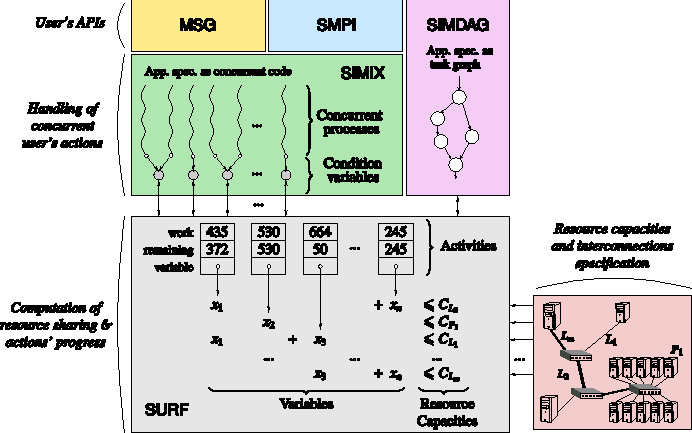
\includegraphics{images/SimGrid.pdf}
		\caption{Architecture of SimGrid \cite{DBLP:journals/jpdc/CasanovaGLQS14}}
		\label{fig:SimGrid}
	\end{center}
\end{figure}
In SimGrid for each simulated activity, such as computation or data transfer, there is a corresponding condition variable, in Figure~\ref{fig:SimGrid} it is shown in SIMIX box. This condition variable synchronizes the concurrent processes of the simulated applications. The computing (\($$P_{x}$$\)) and the communication (\($$L_{x}$$\)) resources are shown on the bottom-right side of the figure. Computing resources are defined in terms of computing power, whereas, communication resources are defined in terms of bandwidth and latency. As shown in the SURF box, multiple activities can share the same resource (e.g., (\($$x_{1}$$\), \($$x_{n}$$\)), (\($$x_{1}$$\), \($$x_{3}$$\)) or (\($$x_{3}$$\), \($$x_{n}$$\))) or one activity can use multiple resources (e.g., \($$x_{1}$$\) or \($$x_{3}$$\) or  \($$x_{n}$$\)). Activities that share the same resource are limited by the capacity of that resource. Each activity is defined by the total and remaining work to be executed. When the work associated with the activity completes, the corresponding upper layer components receive a notification signal \cite{DBLP:journals/jpdc/CasanovaGLQS14}.

As we have already pointed out in Section~\ref{section:packetflow}, the primary advantage of flow-level simulation is its scalability in terms of speed and memory usage. SimGrid uses flow-level analytical model for simulating TCP network phenomenon \cite{DBLP:journals/jpdc/CasanovaGLQS14}. To see the scalability of the flow-level model, the SimGrid team compared it with other widely used simulators such as GridSim and OverSim. After simulating 500,000 tasks both on GridSim and SimGrid, the results demonstrate that SimGrid is 257 times faster and 26 times more memory efficient. Similarly, the comparison result with OverSim shows that SimGrid is 15 times faster and it can also simulate scenarios 10 times larger. Concerning the accuracy, though the simulator gives very good accuracy in most case studies, there are situations where it fails to give accurate result. As an example, the comparison study of SimGrid with packet-level simulator GTNetS show that for data size less than 100 KiB there is a significant difference in prediction. 

Currently SimGrid is used to simulate different network phenomenon in the area of large-scale distributed systems such as grid, cloud, volunteer and HPC \footnote{http://simgrid.gforge.inria.fr/}. Concerning energy consumption models, it houses energy models for CPU but there is no model for network equipments.Therefore, the focus of this study is to propose and implement network energy consumption model for SimGrid. The implementation of this model, together with the existing CPU energy model, allows us to estimate the energy consumption of large-scale networks that reside within or outside a data-center that are discussed in Section~\ref{section:ictequipment} and Section~\ref{section:datacenter}.

\section{Related Simulators}
\subsubsection{ECOFEN}
Orgerie et al.{\ }\cite{DBLP:conf/wowmom/OrgerieLLL11} 
\subsubsection{GreenCloud}
Kliazovich et al.{\ }\cite{DBLP:journals/tjs/KliazovichBK12} proposed GreenCloud, a simulator that can estimate energy consumption of cloud computing data centers. GreenCloud is developed as extension to NS-2 packet-level network simulator. This simulator contains power consumption models both for the computing and communicating components residing in a typical data center. The power consumption model used for the computing component is shown in Equation~\ref{eq:2.4}. This equation contains power consumed by the fixed parts (such as bus, memory and disk) which consume power independent of the operating frequency \emph{f} of the computing component CPU and the power consumed by the CPU (\($$P_f$$\)) operating at a given frequency \emph{f}. This model allows for lowering the operating frequency of the CPU when workload becomes below some predefined threshold in order to decrease the power consumption. 
\begin{equation} \label{eq:2.4}
P_{computing} = P_{fixed} + P_f \times f^3
\end{equation}
The power consumption model used in GreenCloud for the communicating components is the one shown in Equation~\ref{eq:2.3}. The equation shows the static power consuming parts (such as the chassis(\($$P_{chassis}$$\))and the active line cards(\($$P_{linecard}$$\)) and the dynamic part (\($$P_{rate}$$\)), is the energy consumed by the port running at a particular line rate for a given traffic load. 

This simulator is limited in three aspects: number of allowed CPU cores, versatility, and scalability. The first aspect is that only one CPU core is allowed per simulated node. This hinders the study of energy consumption of multi-core computing nodes. The second one is that we can not use this simulator outside the cloud computing domain such as grid, volunteer, peer-to-peer or HPC, at least that is not the authors original intention when they develop this simulator. The available features of the simulators are tuned towards cloud computing applications only. This limits its versatility.

The third aspect deals with the scalability issue. The fine grain details provided by GreenCloud and the packet-level processing approach of the underlying NS-2 simulator is advantageous for getting accurate result when simulating relatively small networks. However, for large-scale distributed networks, it is not scalable. In related to this, the authors have mentioned that their solution gets slower and slower as the number of simulated nodes increases beyond few thousands and as the number of  packets processed increases. In addition to increasing run time, we also expect the memory footprint to increase as the processed packets and the number of simulated nodes increases, even though the authors did not say anything about it.  



\chapter{Environment}
\label{chapter:environment}
In this study we employed SimGrid, ECOFEN, FlowMonitor modules of NS-3 simulator and other tools. This chapter explains the main features of these tools from the perspective of our simulation experiment needs.

\section{SimGrid}
\label{section:simgridenvironment}
In Section~\ref{section:simgrid} of Chapter~\ref{chapter:background} we discussed the software architecture of SimGrid at a higher level. We will give low-level details of the implemented flow-level model and related concepts in later chapter. In this section, our plan is to discuss features of SimGrid that are related to setting up and running energy consumption experiments.

In Figure~\ref{fig:SimGrid} of Chapter~\ref{chapter:background} we have presented three user APIs that SimGrid users can use to develop their simulation experiments. Currently there is another API named S4U that is under development. This API is similar in usage to MSG API. One main difference, from users perspective, is that MSG is in C while S4U is in C++ language. S4U is the API that we have used in this study.  
  
Designing and running simulation experiments in SimGrid using MSG or S4U APIs involve creating three files: a C/C++ simulation Script, an XML file for specifying the simulated platform topology and another XML file for specifying the deployment options, such as, identifying the host that send or receive data, the size of data, and the number of processes sending the data. 

In a typical simulation experiment of energy estimation as a function of data transfer, we can have three sections in the simulation script. In the first section we write a function which specify what the sender do to send the data, in the second section we write what the receiver do to receive the simulated data or what action to take when the simulated data arrives. In the third section we tell to SimGrid's simulation engine about the two functions and we also pass to the engine the platform and the deployment file names. 

In SimGrid, simulated network resources such as, NICs, switches and routers are represented with an abstraction called Link. In SimGrid platform file we represent a Link as follows:

\begin{lstlisting}
<link id="SWITCH1" bandwidth="100MBps" latency="10ms">
      <prop id="watt_range" value="305:550"/>
</link>
\end{lstlisting}

From the link XML tag we can see the basic characteristics of a simulated switch, such as, bandwidth and latency. We also see the idle and busy power consumption range of the switch. Other additional information can also be added such as how the link should be shared when multiple traffic cross the link and tracing information to control the bandwidth and latency property while the simulation is progressing. 

In a similar manner we can specify deployment information such as the role of hosts, the number of processes and the size of transfered data as follows. 
\begin{lstlisting}
<process host="H-1" function="sender">
<argument value="10" />
</process>
<process host="H-2" function="receiver"/>
\end{lstlisting}
This separation of concern among the simulation script, the platform and the deployment configuration files offers great flexibility for designing and running large scale experiments. The platform can be scaled up or down without changing the simulation script, for instance. 

Another feature of SimGrid that we would like to mention here is that SimGrid provides access to NS-3 simulator. This has at least two main advantages. The first one is that for SimGrid users who like to have low level packet information about the simulated network phenomenon, they can launch their experiment from SimGrid interface while using their platform and deployment files that they have created within SimGrid. The second one is that for studies similar to ours this feature helps a lot during the validation process of newly implemented model. This feature allowed us to run the validation comparisons with NS-3 using the same platform and deployment file that we have created in SimGrid. SimGrid automatically maps the topology and the corresponding parameters into NS-3's abstraction.
\section{NS-3}
NS-3 is a discrete-event packet-level simulator, events corresponding to, for instance, arrival and departure of packets. NS-3 is structured in a modular manner. The core and the network modules are two of the modules that serve as generic simulation core that can be used for Internet-based or different network type simulation. These two modules, being generic, are independent from any device models. The core module provides features such as tracing, callbacks, smart pointer, random variables, events and schedules. The network module consists components such as packets, node, addresses (e.g.,~IPv4 and MAC) and network devices. The components provided by the simulation core modules can be used to create other modules. This feature allows researchers to add their own models for the network phenomenon that they want to simulate. We will visit two of the modules that are constructed in this way in the next two subsections\cite{ns3}. 

The NS-3 core and other modules are built in C++ language as a set of libraries. The user can access these libraries in their main C++ program to configure the simulated topology and other simulator parameters. The libraries are also available as Python API for those researchers who prefer Python programming language. 

\subsection{ECOFEN Module}
ECOFEN is one of the two non-core NS-3 modules that we used in our experiments. We explained the power consumption simulation features provided by this module in the Related Simulators section of Chapter~\ref{chapter:background} and we will give detailed explanation about why and where we have used it in our Method chapter. In this section, we only give brief description about how it is related to NS-3 and how we have used it. 

NS-3 in its core provides an abstraction such as Node, Net Device, Channel and Application. A Node represents  network communication and computing devices (currently NS-3 do not have CPU abstraction) such as servers, switches and routers. To a Node a Net Device, which represent devices such as network interface card (NIC), can be attached. Two or more Nodes can be linked to each other through a Channel, which is a representation of Ethernet or Wi-Fi link. These three abstractions: Node, Net Device, and Channel, together they can be used to define the simulated network topology. Application, on the other hand, is an abstraction that represent user program that perform some simulated activity such as sending or receiving UDP packets~\cite{ns3}. 

Using the core abstractions provided by NS-3, such as  Node, Net Device, and Packet, the ECOFEN module implemented three power consumption models that enable users to simulate power consumption as a consequence of packets transmission at different levels of granularity as discussed in Chapter~\ref{chapter:background} and Chapter~\ref{chapter:methods}.

In a typical NS-3 simulator script, in its main function, we can recognize four common sections: (1) the section where we find statements that import the required core or other modules, (2) the section where the topology of the simulated network is defined, (3) the section where the simulated user application is defined, and (4) the section where statements related to running, starting, stopping and cleaning the simulation is specified. This is a rough approximation, certainly there are other statements such as those that are related to logging and tracing. 

The NS-3 scripts that we used in our power consumption simulation experiments imported the ECOFEN module in their first section, set up and configured the energy consumption models in the second section, configured an application that send and receive UDP or TCP packets in the third section, and finally, in the fourth section, we stated when the simulation should start and end. 

\subsection{FlowMonitor Module}
FlowMonitor is the other non-core NS-3 module that we have employed in our study. This module is designed with the aim of providing generic network traffic inspection facility. It provides researchers, who want to measure the simulated network efficiency, with standard performance metrics such as bit-rate, duration, delay, packet-size and packet loss ratio~\cite{DBLP:conf/valuetools/CarneiroFR09}.  

Among the performance metrics that are available in FlowMonitor module, the following are the ones that we have used in our simulation experiments.
\begin{itemize}
	\item \textbf{\textit{rxBytes}} to get the received bytes by a node,
	\item \textbf{\textit{txPackets}} to get the transmitted packets by a node,
	\item \textbf{\textit{timeFirstRxPacket}} and \textbf{\textit{timeLastRxPacket}} to get the absolute time when the first packet and the last packets in the flow was received,
	\item  \textbf{\textit{timeFirstTxPacket}} and \textbf{\textit{timeLastTxPacket}} to get the absolute time when the first and last packets in the flow was transferred and 
	\item \textbf{\textit{lostPackets}} to check if there are lost packets.
\end{itemize}
We used the above performance metrics to compute throughput (T) with the unit of Mega-bits per second (Mbps) and Packets per second(Pps) as shown in Equation~\ref{eq:3.1} and Equation~\ref{eq:3.2}. 
\begin{equation} \label{eq:3.1}
\begin{split}
T_{Mbps} &= rxBytes \times 8.0 \times 10^{-6} /\\
  & (timeLastRxPacket - timeFirstRxPacket)
\end{split}
\end{equation}
\begin{equation} \label{eq:3.2}
T_{Pps} = txPackets / (timeLastTxPacket - timeFirstTxPacket)
\end{equation}
\section{Other tools}
We followed, partly, the literate programming and reproducible research approach proposed in~\cite{DBLP:journals/sigops/StanisicLD15,schulte2012multi}. In this approach, the authors used two well-known tools: Git and Org-mode. A Git branching model is proposed in~\cite{DBLP:journals/sigops/StanisicLD15} that ease the synchronization of data and the code that generated the data. Org-mode, on the other hand, is employed as a literate programming tool for managing a laboratory notebook.  

Org-mode\footnote{http://orgmode.org/} is a plain text mark-up language which is available as an extension to Emacs text editor. An Org-mode document can have different sections: a plain text, an executable code block and/or a data block. The code and the data blocks are active, meaning they can be evaluated (or executed) and as a result they can output the code or the data block as passive (plain text) form and/or the computational result of the evaluated code or the data block. This feature allows Org-mode to be a powerful tool for literate programming.

Whenever we wanted to do some experiment, we used Org-mode in our laboratory notebook to capture the experimental environment, such as, the objective of the experiment, the assumptions we made, the parameters used, the links referenced, and any other information relevant to our experiment. Within the same document we also put chunks of codes wherever we want them using programming languages such as bash shell, python, and R. What is more amazing is that Org-mode allowed us to name and call the executable codes from anywhere within the document with different input parameters, hence we were able to reuse previously written code blocks. 

We used the shell script to run NS-3 and SimGrid simulation scripts and also to capture their outputs. We used Python to extract and format the data we want from the raw data produced by the simulators. Then we used R with its ggplot2 package to generate different plots and to do statistical analysis.




\chapter{Methods}
\label{chapter:methods}

In this chapter we begin by first describing the common approaches followed by researchers for a variety of energy consumption experiments, their advantages and disadvantages. Then we present the approach we followed for our study and its justification.
\section{Common Approaches}
\label{section:commonappraoches}
One approach for estimating energy consumption of a given network is by employing actual power meter to measure the power drawn by involved network and computing components. A good example for such case is the measurement that Fan and his team conducted~\cite{DBLP:conf/isca/FanWB07}. In this study the authors have managed to monitor power consumption of several thousand of servers over a period of six months on real live workload. Mahadevan et al.,~in~\cite{DBLP:conf/networking/MahadevanSBR09}, have also done a similar power measurement on a production environment for studying power consumption behavior of networking devices such as switches and routers. If the measurements are done correctly, this approach produces the most real picture of the network under investigation compared to the other two approaches that we will discuss in subsequent paragraphs. However, this approach has certain inherent drawbacks. First, real production networks might not be available for experimentation. Even if they become available, the transient and varying nature of the production environment makes it hard to repeat the experiments. Second, we have little or no control over factors affecting the measured power consumption. We do not have the privilege of injecting or modifying the traffic or the workload in order to test different experimental hypothesis. To have a full control we need another approach. 

Experimental testbed is another approach that researchers have used to study power consumption characteristics of different computing and networking devices. In this approach first a separate network is setup and configured solely for the purpose of conducting experiments. Then researchers make measurements by manipulating factors that affect power consumption according to the hypothesis that they want to test. Unlike the previous one, this approach offers greater flexibility over the experimental parameters. In the power measurement study scenario that we are discussing, the researcher can change parameters such as traffic rate, packet size, inter-packet time interval and transmission protocol used (TCP/UDP). Sivaraman et al.~in~\cite{Sivaraman} have setup experimental testbed for determining per-packet processing and per-byte receipt, storage, queuing, and transmission power consumption. The experiment setup involved hardware-based traffic generator (which gives fine grain control over parameters such as the packet size, inter-packet interval and data rate), NetFPGA\footnote{http://www.netfpga.org/} experimental router and digital oscilloscope for measuring the power draw of the NetFPGA router. A similar experiment but with commercial switches of different vendors is explained in~\cite{DBLP:journals/comcom/SivaramanRZSVMR14}. The primary advantages of this approach is that the researcher can have full control over the experimental parameters provided by the tools involved in the testbed and experimental result can also be very accurate. The first disadvantage though is that it can easily become very expensive when we want to experiment on large-scale level. The second disadvantage is that experimenting on different scenario might require considerable reconfiguration and even a completely new testbed, which apart from limiting the flexibility, it can also be very costly, time and effort consuming. We need an approach which overcome these shortcomings. That is, we need an approach which gives full control over the experiment, which is reasonably accurate, less expensive and very flexible. 

Simulation is the most widely used approach in computer network research~\cite{DBLP:conf/icc/WeingartnerLW09}. It has several advantage compared to the other two approaches mentioned before. First, it makes it relatively easy, for instance, the study of the performance of non-existing network protocol or algorithm. One can propose and validate, by simulation experiment, a new energy-aware routing protocol or algorithm for wired or wireless networks. This is what Swain et al.~\cite{DBLP:conf/aina/SwainHC10} did in their new energy-aware routing protocol proposal for wireless sensor networks. Second, though it depend on the design of the particular simulator used, in general, simulation approach allows running large scale experiments that involve hundreds and thousands of nodes with less effort and cost compared to the other two approaches. In~\cite{DBLP:conf/wowmom/OrgerieLLL11} and~\cite{DBLP:conf/cloudnet/CorneaOL14}, the NS-3 module, ECOFEN, is used to simulate energy consumption of large-scale networks with nodes more than 600 and 1000, respectively. In~\cite{DBLP:journals/tjs/KliazovichBK12} Kliazovich et al.~studied energy consumption of data center networks with two-tier and three-tire architectures that encompasses 1536 nodes. Third, in simulation scaling does not incur monetary cost, though it is limited by performance factors such as runtime and memory usage~\cite{DBLP:conf/icc/WeingartnerLW09}. Fourth, the researcher has great flexibility and full control over the simulation experiment. Finally, simulators makes output data management extremely easy by providing mechanisms such as logging, tracing and visualization~\cite{ns3,DBLP:journals/jpdc/CasanovaGLQS14}.  

Though simulation experiment has quite a lot of advantages over experiments done on production environment or experimental testbeds, it faces one big challenge, accuracy. In the process of approximating the real network phenomenon in the simulation model, some less significant concepts are abstracted away, for instance, to reduce complexity or to gain performance improvement, which results in unavoidable loss of accuracy. However, in other instances the models used in a given simulator might fail to correctly capture the simulated real network phenomenon. In~\cite{DBLP:journals/tomacs/VelhoSCL13} the authors demonstrated incorrect modelings found in popular simulators such as OptorSim, GridSim and CloudSim. Therefore, (in)validating the correctness of a simulator is important task that should be undertaken before any simulation experiment for two related reasons. Either to know the boundaries within which the simulator used produce reasonably accurate results, or to know if the simulator produce the expected or the correct result. The validation can be done either by comparing the output of the simulator against accurate measurements obtained from real networks or by comparing the output against another simulator whose accuracy is already known~\cite{DBLP:books/daglib/0076234}.
\section{Our Approach}
\label{section:ourapproach}
The goal of this study is to investigate the accuracy and scalability of flow-level models, as compared to packet-level models, in estimating energy consumption of large-scale distributed networks. To achieve this goal, we first search literature to find and propose a suitable flow-level model. Second, we implement the model in SimGrid. Finally, we run different experiments to test the accuracy and the scalability of the implemented flow-level model by comparing it against a packet-level model. For our experiments, we chose the simulation approach among the three alternatives discussed above. 

Before describing the details of our approach, let us first justify why we end up with the relatively complex method shown in Figure~\ref{fig:approach}. There is experimental test-bed (Grid'5000\footnote{https://www.grid5000.fr/mediawiki/index.php/Grid5000:Home}) in France that we have access to. Grid'5000 is experimental test-bed specifically designed for studying large-scale distributed networks~\cite{DBLP:journals/ijhpca/BolzeCCDDJJLLMMNPQRTT06}. However, we could not used it for our purpose (i.e., for studying large-scale flow-level relationship of power consumption and traffic) as the network devices are not equipped with power meters accurate enough (current power meters on Lyon site of Grid'5000 provide one measurement per node and per second). As a result, we opted to use a packet-level simulator with power consumption models obtained from literature. Subsequent paragraphs describe the specific steps we followed in our approach.

As we have discussed in Chapter~\ref{chapter:background}, SimGrid already have energy consumption model for CPU which corresponds to the computing part of a given large-scale network. What we wanted to add is energy consumption model for communication components such as switches and routers. Therefore, the initial task in our approach is to study literatures (\circled{A} in Figure~\ref{fig:approach}) in order to find and propose a model which describe the power consumption characteristics of communication equipments such as switches and routers. Our search returned the linear relationship that we have described in Equation~\ref{eq:2.2}~\cite{Sivaraman,DBLP:journals/comcom/BeisterDAK14,DBLP:conf/networking/MahadevanSBR09,DBLP:conf/sigcomm/MahadevanBS10}. This equation tells us that the power consumption of a network equipment constitutes the idle and dynamic components. The idle power consumption represents the power drawn by the equipment while it is on but with no traffic. The dynamic consumption, on the other hand, represent the additional power drawn due to network traffic. The next task (\circled{C} in Figure~\ref{fig:approach}) is to implement this linear model for SimGrid and (in)validate its accuracy against ECOFEN module (\circled{D} in Figure~\ref{fig:approach})~\cite{DBLP:conf/wowmom/OrgerieLLL11,DBLP:conf/cloudnet/CorneaOL14}. This task is done iteratively by switching between model implementation and accuracy validation. The final task (\circled{G} in Figure~\ref{fig:approach}) is to show the scalability of the implemented flow-level model against the existing packet-level model in ECOFEN. For this, we designed and run two kinds of experiments (\circled{E} and \circled{F} in Figure~\ref{fig:approach}), one for speed and one for memory usage. 

The purpose of the accuracy and the scalability experiments shown in \circled{D} and \circled{G} in Figure~\ref{fig:approach} is to test our \emph{hypothesis}, which states: \emph{flow-level energy consumption models can give reasonably accurate estimation and they can also be significantly more scalable than packet-level models}. 

We chose to use ECOFEN as packet-level simulator to compare the accuracy and performance of the implemented model for two primary limitations that exist in the other alternative simulator, GreenCloud~\cite{DBLP:journals/tjs/KliazovichBK12}. The first limitation is that GreenCloud is designed for a  cloud computing environment. This is in contrary to one of SimGrid's main design principles, versatility~\cite{DBLP:journals/jpdc/CasanovaGLQS14}. ECOFEN, on the other hand, is not tied to one particular large-scale networking paradigm, therefore, suits more for our purpose. The second limitation of GreenCloud is that it is build on top of currently obsolete NS-2 simulator. In comparison, though ECOFEN was also initially built as NS-2 simulator module, currently it is rewritten for NS-3~\cite{DBLP:conf/cloudnet/CorneaOL14}. One of the major advantage of using NS-3 over NS-2 is that NS-3 performs considerably better in both runtime and memory-usage metrics~\cite{DBLP:conf/icc/WeingartnerLW09}.

In the accuracy-validation and scalability-comparison experiments mentioned in our approach, we are comparing the newly implemented flow-level model in SimGrid simulator against another packet-level simulator model implemented in ECOFEN module. This simulator-to-simulator comparison is valid only if the later simulator model, against which the new implementation is to be validated, is known to be accurate. However, we could not find any information that tell us the accuracy of the ECOFEN module. Therefore, we designed a validation experiment (\circled{B} in Figure~\ref{fig:approach}) for ECOFEN as described in the next section. 
\begin{figure}[ht]
	\begin{center}
		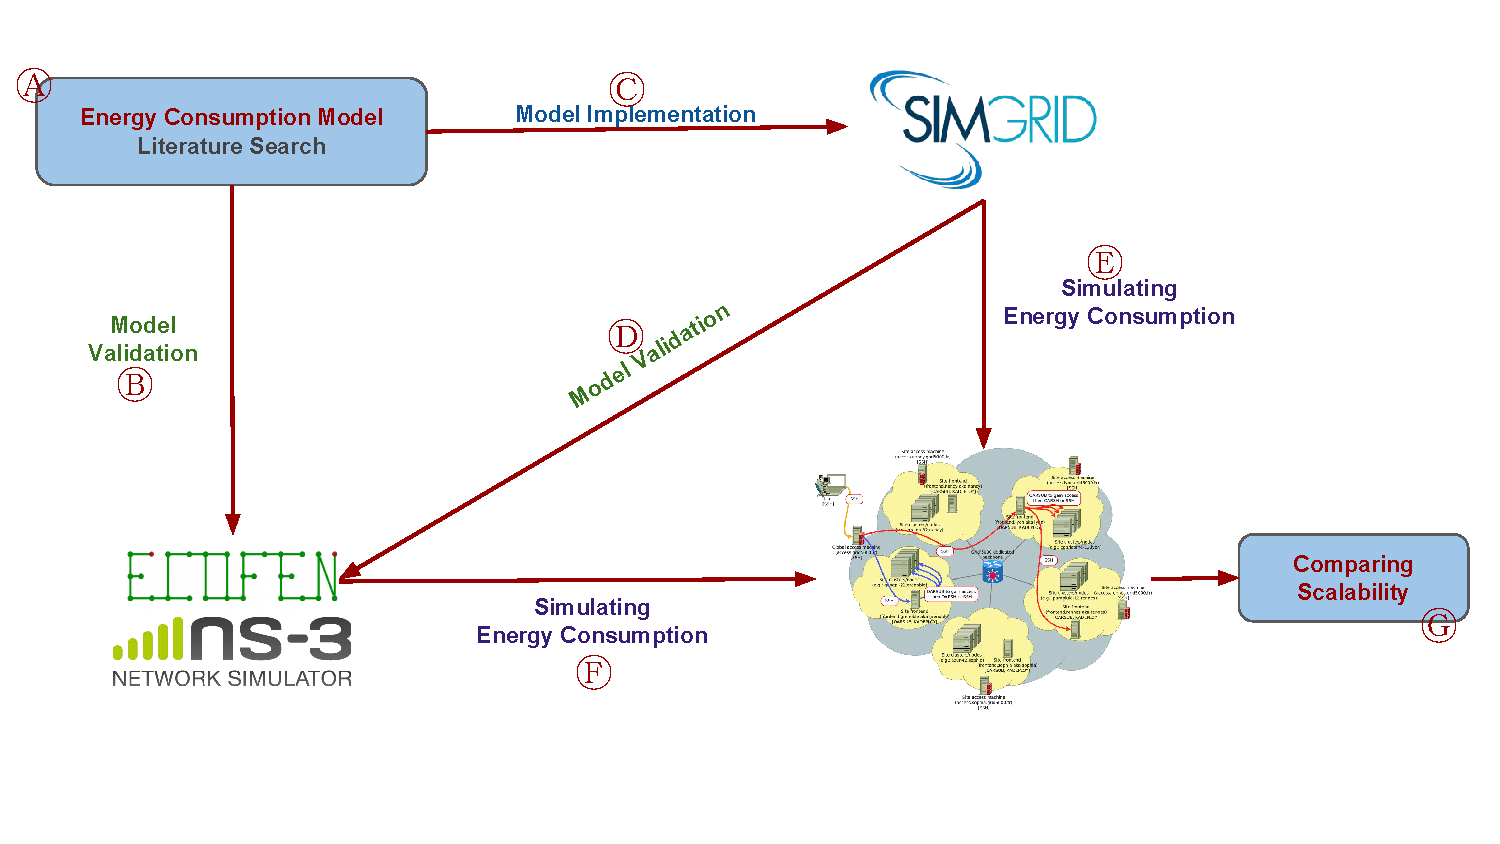
\includegraphics[width=13cm]{images/approach.pdf}
		\vspace*{-1.0cm}
		\caption{Summary of the experimental method we followed in this study}
		\label{fig:approach}
	\end{center}
\end{figure}
\section{Validating ECOFEN}
ECOFEN has three models with names \emph{basic}, \emph{linear} and \emph{complete} that we have discussed in Section~\ref{section:relatedsimulator} of Chapter~\ref{chapter:background}. Both the \emph{linear} and \emph{complete} models can produce values of power consumption as a function of traffic. The  \emph{basic} model, on the other hand, produces power consumption values based on the ON or OFF state of a node, it does not consider network traffic. Therefore we describe the validation experiments for both the \emph{linear} and the \emph{complete} models in this section. 
 
The basic procedure for the validation experiment is first to simulate, using ECOFEN, power consumption in response to traffic sent or received and then to compare the results against data obtained from literature where actual measurement is conducted.

\subsubsection{Validating the Linear Model}
In the work of Sivaraman et al.~\cite{Sivaraman} we can find the result of a power consumption experiment that is shown in Figure~\ref{fig:powervsdatarate1}. The figure displays the linear relationship that exist between traffic volume (in Mbps) and power consumption (in watts) for a fixed packet sizes of 100, 576, 1000, and 1500 bytes. Furthermore, in the figure, the linear fit equations (models) for each of the packet sizes are also displayed. 

The authors intention in this experiment is to determine values of the per-byte and the per-packet processing energy consumption, however, our intention is to use the per-byte energy consumption value that they have experimentally determined and to use it in ECOFEN to get power consumption values for a given volume of traffic. Then compare the results we obtained with the linear fit models that are shown in Figure~\ref{fig:powervsdatarate1}. The linear fit equations shown in Figure~\ref{fig:powervsdatarate1} are derived from actual power measurements.

In their experiment, the authors used three kinds of hardware devices: (1) NetFPGA router card that has four 1 Gbps Ethernet ports, (2) IXIA hardware traffic-generator for generating packets with the desired packet-size and data-rate, and (3) high-fidelity oscilloscope for measuring the power consumed by the NetFPGA card as a consequence of the packets send or received. 

\begin{figure}[ht]
	\begin{center}
		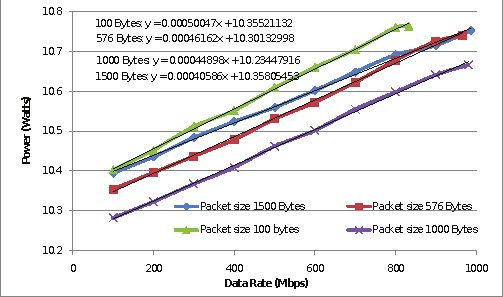
\includegraphics[width=13cm]{images/powervsdatarate1.pdf}
		\caption{Power consumption vs data-rate for fixed packet size from~\cite{Sivaraman}.}
		\label{fig:powervsdatarate1}
	\end{center}
\end{figure}

The linear model of ECOFEN module accepts energy consumption values for the idle state of a simulated network interface card (NIC) and the per-byte processing. The underlying NS-3 platform, in addition, provides us with more parameters such as packet-size and data-rate, which among other parameters, enable us to have full control over the generated traffic.

In this validation experiment we wish to simulate the experiments conducted by Sivaraman et al.~as closely as possible. With this in mind, we setup, in our NS-3 simulation script, a three node simple network with first and third nodes connected to the second node. All the three nodes are connected to each other by links that have maximum bandwidth capacity of 1 Gbps and delay of 10 ms. 

We got the idle consumption values for each of the packet-size models shown in Figure~\ref{fig:powervsdatarate1} by setting the x component (the data rate value) of the equations to zero and for a per-byte processing energy consumption value we used 3.4 nJ. This is the value that the researchers experimentally determined. 

For the generated traffic volume in the simulation, we used uniform random number generator provided by NS-3 in order to get integer values between 1 and 1000. Our NS-3 script, in addition to packet-size and data-rate values, also requires number of packets to be send and also inter-packet interval time values. These values are derived from packet-size and data-rate parameters. 

Since there might be unexpected results, for instance, due to wrong network configuration, we have employed NS-3's FlowMonitor module to monitor the actual traffic transfered in the simulated network. Using this flow monitoring module, we have confirmed if all the traffic generated by the sending end are also received at the receiving end. We have also used this module to compute the actual traffic rate (throughput) both at the receiving and the sending ends as shown in Equation~\ref{eq:3.1} and Equation~\ref{eq:3.2} in Chapter~\ref{chapter:environment}.

Finally, we set the remaining simulation environment configuration settings such as starting and stopping time and then run the experiment 40 times, each time with different run value for the random number generator. The result obtained is depicted in Figure~\ref{fig:linear}. In the graph the expected power consumption values from the linear fit models shown in Figure~\ref{fig:powervsdatarate1} along with the simulated values for each of the packet sizes (100, 576, 1000, and 1500 bytes) are displayed.

Visually, the simulated and the expected values seem to agree very well, even though the gap between them starts to grow slightly larger (especially when the packet size is 100 bytes) for larger data-rates. In order to be more sure, we run unpaired t-test statistical test using the produced data. The summary of this test is shown in Table~\ref{table:linearttest}. 

The 95\% confidence interval values shown in Table~\ref{table:linearttest} of difference in mean between the measured and simulated values are very close to zero and in fact zero is also one of the values. The P-values are also confirming the same thing, the null hypothesis that the difference in mean between the simulated and the expected values is zero is not rejected. 
\begin{figure}[ht]
	\begin{center}
		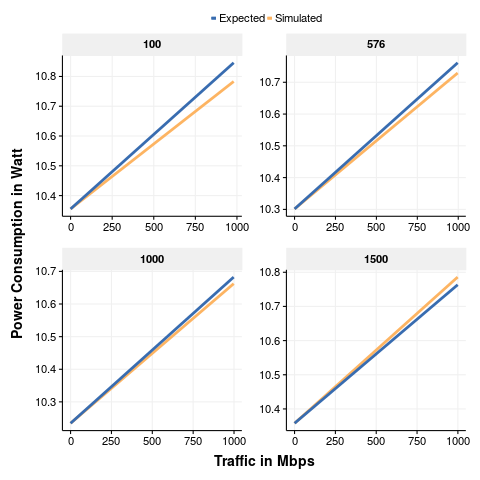
\includegraphics[width=13cm]{images/expectedvssimulatedlinear.png}
		\caption{Power consumption vs data-rate comparison between expected (or measured) values (in red color) and simulated values (in light blue color) for a fixed packet size of 100, 576, 1000, and 1500 Bytes}.
		\label{fig:linear}
	\end{center}
\end{figure}
\begin{table}
	\begin{tabular}{|>{\centering\arraybackslash}m{1.3cm}|>{\centering\arraybackslash}m{4.2cm}|>{\centering\arraybackslash}m{2.1cm}|>{\centering\arraybackslash}m{2.1cm}|>{\centering\arraybackslash}m{1.3cm}|} 
	    \hline 
		\textbf{Packet Size} & \textbf{Confidence Interval of difference in mean} & \textbf{Mean of Expected} & \textbf{Mean of Simulated}& \textbf{P-Value}\\ 
		\hline 
		 100 &[-0.027, 0.110]&10.640&10.599&0.230\\
		\hline
		 576 &[-0.039, 0.082]&10.544&10.523&0.480\\ 
		\hline
		 1000&[-0.043, 0.073]&10.466&10.451&0.6131\\ 
	    \hline	 
	     1500&[-0.062, 0.048]&10.566&10.573&0.796\\ 
	    \hline
	\end{tabular} 
	\caption{Unpaired t-test results for simulated and measured power consumption values for ECOFEN's linear}
	\label{table:linearttest}
\end{table}

The conclusion in this validation test is that the linear model of ECOFEN is accurate in predicting the power consumed by NetFPGA router for a given volume of traffic. 

\subsubsection{Validating the Complete Model}
Roughly, in this validation experiment, we have used the same experimental configuration and procedure as that of the linear validation experiment that we have described in the previous section. Therefore, in this section our focus is more on the result than on the configuration.

One of the main difference between the complete and the linear model of ECOFEN is that the complete model distinguishes between the received and sent bytes. Which means that different energy consumption values can be assigned to bytes based on the direction of transfer. The linear model, on the other hand, assigns same value for both. The other main difference is that the complete model considers the packet processing energy consumption cost both for the sent and received packets. 

Sivaraman et al.{\ }\cite{Sivaraman} also conducted experiments to determine energy consumption values for per-byte receive or transmit and per-packet processing. The experimentally determined values for per-byte receive is 1.3 nJ, for per-byte transmit is 2.1 nJ, and for per-packet processing is 197.2nJ. 

We have slightly modified the NS-3 script that we have used in the previous section to make it suitable for this experiment. Now we have configured our script for the ECOFEN's complete model to use energy consumption values for per-byte receive or send and per-packet processing. Further more, we have upgraded the link capacity between the nodes from 1 Gbps to 2 Gbps. Finally, we set the traffic rate in terms of packets per second in the sending end and in terms of Mbps in the receiving end in order to comply with the experiments done by mentioned authors. The results for the sending and receiving are is shown in Figure~\ref{fig:sending} and Figure~\ref{fig:receiving}, respectively. The linear fit models we have used for this validation experiment are also available in \cite{Sivaraman}. There is only one linear fit model (for packet size 1000 bytes) for the sending end and there are three for the receiving end.   
\begin{figure}[ht]
	\begin{center}
		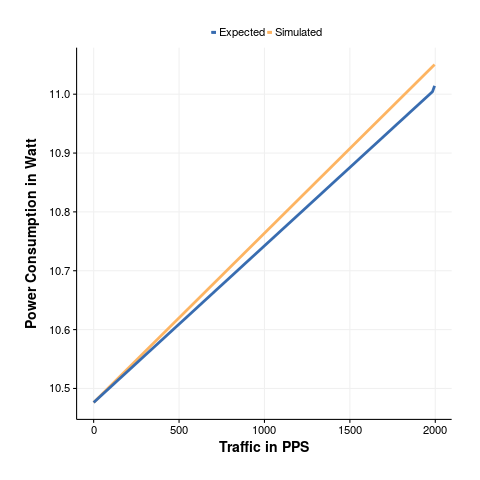
\includegraphics[width=11cm]{images/expectedvssimulatedsending.png}
		\caption{Power consumption vs data-rate comparison between expected (or measured) values (in red color) and simulated values (in light blue color) for a fixed packet size of 1000 Bytes for the sending end}
		\label{fig:sending}
	\end{center}
\end{figure}
\begin{figure}[ht]
	\begin{center}
		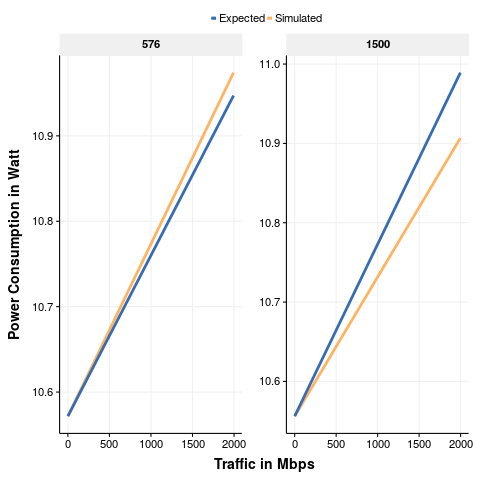
\includegraphics[width=11cm]{images/expectedvssimulatedreceiving.png}
		\caption{Power consumption vs data-rate comparison between expected (or measured) values (in red color) and simulated values (in light blue color) for a fixed packet size of 576 and 1500 Bytes for the receiving end}
		\label{fig:receiving}
	\end{center}
\end{figure}
Table~\ref{table:complettest} shows the unpaired t-test result for one packet-sizes in the transmitting side (Tx) and for two packet-sizes in the receiving side (Rx). 
\begin{table}
	\begin{tabular}{|>{\centering\arraybackslash}m{1.3cm}|>{\centering\arraybackslash}m{0.7cm}|>{\centering\arraybackslash}m{3.9cm}|>{\centering\arraybackslash}m{2.1cm}|>{\centering\arraybackslash}m{2.1cm}|>{\centering\arraybackslash}m{1.2cm}|} 
		\hline 
		\textbf{Packet Size} & End &\textbf{Confidence Interval of difference in mean} & \textbf{Mean of Expected} & \textbf{Mean of Simulated}& \textbf{P-Value}\\ 
		\hline 
		576 &	Rx&[-0.067, 0.039]&         10.770 &          10.784&   0.598 \\
		\hline
		1500&	Rx&	[-0.010, 0.095] &        10.778 &         10.736& 0.114\\ 
		\hline
		1000&	Tx&	[-0.096, 0.053] &        10.750 &         10.773 & 0.560 \\ 
		\hline	 
	\end{tabular} 
	\caption{Unpaired t-test results for simulated and measured power consumption values for ECOFEN's complete model}
	\label{table:complettest}
\end{table}

Again in this case the 95\% confidence interval values shown in Table~\ref{table:complettest} of difference in mean between the measured and simulated values are very close to zero and in fact zero is also one of the values. The P-values are also confirming the same thing, the null hypothesis that the difference in mean between the measured and the simulated values is zero is not rejected. 

The conclusion from this validation experiment is also the same as the previous one, the ECOFEN's complete energy consumption model accurately predicts power consumed by NetFPGA router for a given volume of sent or received traffic.  

 


 
\chapter{Implementing flow-level model}
\label{chapter:implementation}

In this chapter we start by describing how we started the implementation task, we then move to the discussion of the implementation details together with the challenges we encountered. Finally, we present the final version of the implemented flow-level model. 
\section{The starting flow-level model}
By definition, as we have shown in Equation~\ref{eq:2.1}, the energy consumption of a given electronic equipment is given by the product of the average power drawn by the equipment and its time duration of running. We have also shown, in Figure~\ref{fig:energyproportionality} and Equation~\ref{eq:2.2}, the linear relationship that exist between network equipment load and power consumption. Combining Equation~\ref{eq:2.1} and Equation~\ref{eq:2.2}, we get the following equation for energy consumption for a given time duration of T, where \($$P_{idle}$$\) is the power that the equipment consumed when there is no traffic and \(P_{dynamic (avg)}\) is the average power drawn during the time interval T in the presence of network traffic.

\begin{equation} \label{eq:5.1}
E(T) = (P_{idle} + P_{dynamic (avg)}) * T 
\end{equation} 

To implement this model in SimGrid, we need to determine the values of the three variables shown in Equation~\ref{eq:5.1}. We can directly read the idle power consumption value from the SimGrid's link property that we described in Section~\ref{section:simgridenvironment}. For the other two, we need to understand how SimGrid compute load and time in its core. 

Briefly described, for a set of simulated activities running on a given simulated resource such as a switch, SimGrid computes using its MAX-MIN algorithm the amount of resource that each activity can get. At a given moment the sum of the resources that are assigned to all activities running on the resource cannot exceed the capacity of the resource. Figure~\ref{fig:SimGrid} depicts this concept symbolically and we can access how much of the resource is currently in use, i.e., its load. 

In our case, the load is the total amount of bandwidth that is assigned to all data transfer activities running on a given Link and we can get the maximum bandwidth capacity of the Link from its description on the platform file. With these two information and with the busy power consumption value of the link, we can compute the dynamic power consumption part of the Link at a given instant, \(P_{dynamic}\), as shown in Equation~\ref{eq:5.2}:

\begin{equation} \label{eq:5.2}
P_{dynamic} = (P_{busy} - P_{idle}) * u 
\end{equation} 
where:
\begin{description}
    \item [u]: is a normalized utilization factor obtained by dividing the current Link load with its full capacity, and 
    \item [(\($$P_{busy} - P_{idle}$$\))]: is the slope of the relationship between load and power consumption as shown in Figure~\ref{fig:energyproportionality}.
\end{description} 

Now we are left with computing the time, T, variable of Equation~\ref{eq:5.1}. We can get this value from SimGrid, we can read the current time value, for example, when a given data transfer completes and then use that value to compute the energy consumed to transfer the data.

We implemented this model and designed a simple simulation experiment with two nodes connected by a single link. The link has a fixed bandwidth (1 GBytes) and a fixed latency (10 ms). We then run this experiment in both SimGrid and ECOFEN module of NS-3 40 times with randomly generated data size values between 1 and 1000 MBytes. From the simulation output we have realized that there is a significant difference between ECOFEN's and SimGrid's output in terms of the simulated time required to transfer a given size of data. 

The approach we followed to resolve this issue is to obtain an equation which relate data transfer time with data size. Sine we are using ECOFEN module of NS-3 (a packet-level simulator) as a ground truth, we used it to study the relationship between data transfer time and data size. We got, using R, the linear relationship \($$T_{A}$$\) shown in Equation~\ref{eq:5.3}, with the estimated value of parameter \($$\beta_1$$\) and \($$\beta_2$$\) being approximately 0.153 and 0.65. We did this parameter estimation experiment with fixed value of bandwidth and latency.
\begin{equation} \label{eq:5.3}
T_{transfer} = \beta_1 * data\_size + \beta_2
\end{equation} 
With the data transfer time equations included, our revised model is shown in Equation~\ref{eq:5.5}.
\begin{equation} \label{eq:5.5}
E(T) = (P_{idle} + (P_{busy} - P_{idle}) * u ) * T_{transfer}
\end{equation} 
where:
\begin{description}
	\item [\($$T_{transfer}$$\)] = \($$0.1526 \times data\_size +0.6513248$$\), and 
\end{description} 
We revised our implementation with this modification. Using the load (used bandwidth of a link in bytes/sec) that SimGrid computes for each link, we computed the transfered data (bytes) for our data\_size variable in Equation~\ref{eq:5.5}. Since SimGrid recomputes the load of each link whenever there is network activity event, we collected the bytes at each event change by multiplying used bandwidth of a link by time duration elapsed between the last event and the current one. Then we got \($$T_{transfer}$$\) for the total bytes transferred when simulation end event occurs. 
\section{The final model}



\chapter{Validation}
\label{chapter:evaluation}
In this chapter we present the accuracy and the scalability experiments we performed to evaluate the implemented flow-level model. As we outlined in our method chapter, we compare our implementation with the packet-level implementation of ECOFEN (based on NS-3).  
\section{Experiment Setup}
For all our experiments the version of NS-3 we used is version 3.26 and that of SimGrid is version 3.15. 
\subsection{General ECOFEN related setup}
Among the three power consumption models available in ECOFEN module, we used the \emph{linear} one. This model accepts idle power consumption values in Watts and also energy consumption values for each Byte received or send in nanoJoule. Throughout our experiments we used 10.3581 Watt as idle power consumption value and 3.423 nJ as Byte energy consumption value. We took these values from \cite{Sivaraman}, even though any arbitrary values can also suffice for our purpose.

\todo[inline]{You could specify here for which network device these values have been measured.} 

The linear model estimates power consumption value based on these two inputs and the amount of transmitted or received traffic and then display the estimated power consumption in Watt at specified time interval. We set the interval to be 0.05 sec (20 estimations per second) in order to get more frequent power estimation. 

What we want to get from ECOFEN is the total amount of energy consumed by the simulated network. To get this value, we first compute the average power drawn by the network for a given data transfer task and when the task ends, we multiply the average total network power with the data transfer time. 

\subsection{General SimGrid related setup}
For all of our experiments we used a simple client/server SimGrid application. As described in Chapter~\ref{chapter:environment}, a typical SimGrid script contains three sections. Accordingly in our script, the first section represents what the client function does to send data. It simply accepts the number of Bytes to send from command line option or uses a default 1,000 Bytes if no value is specified, or it will generate the Bytes if random option is specified in the command line. Then it passes the Bytes to the SimGrid's send routine. By default there will be only one TCP flow for the specified Bytes, but if we want to send multiple flows we can specify the number of flows on the command line. The server function simply issues the receive routine if there is data to receive. The third section, in addition to doing the tasks specified in Chapter~\ref{chapter:environment},  it is also a gateway to NS-3 or our implemented flow-level model depending on the option specified in the command line. 

For the Link tag in SimGrid's platform file we used 10 Mbps  as a bandwidth value. This value is chosen because it falls within the range where ECOFEN's and SimGrid's simulated time value match closely as we have described by the end of Chapter~\ref{chapter:implementation}. For latency we used 10 ms and as a Watt-range power consumption value, we used 10.3581 Watt as idle power consumption value and 10.7479 Watt as a busy power consumption value. 

SimGrid's interface to NS-3 will set these bandwidth and latency values, together with other parameters, to NS-3's configuration automatically. It means that we have only one SimGrid script to run both simulations (flow-based in SimGrid directly and packet-level in NS-3 with ECOFEN), thus ensuring a fair comparison on the same simulated network with the same generated traffic. 

\section{Accuracy Validation}
Our first objective consists in evaluating the accuracy of SimGrid's energy consumption estimates (done with our energy flow-based model) against the values computed by ECOFEN.
For this accuracy validation, we conduct two sets of experiments. In the first set, our purpose is to investigate the accuracy of energy consumption estimation difference between ECOFEN and the flow-level model when the size of platform changes. In SimGrid case, it means when the number of Links change; in ECOFEN case, when the number of Nodes, NetDevices and the connection between them change. For this experiment we keep the number of flows and the data volume fixed but we increase the number of Links. In the second set, on the other hand, our purpose is to study the difference between the estimated energy consumption value between ECOFEN and SimGrid when the data size or flow changes while keeping the number of links fixed. Table~\ref{table:accuracyscenarios} shows all the tested scenarios and Figure~\ref{fig:sgvsns3scenario} shows the energy consumption prediction behavior of the implemented model and ECOFEN's model for all of the scenarios summarized in Table~\ref{table:accuracyscenarios}.

\begin{table}
	\begin{tabular}{|>{\centering\arraybackslash}m{1.6cm}|>{\centering\arraybackslash}m{1.8cm}|>{\centering\arraybackslash}m{1.9cm}|>{\centering\arraybackslash}m{1.8cm}|>{\centering\arraybackslash}m{2.2cm}|>{\centering\arraybackslash}m{1.6cm}|} 
		\hline 
	\textbf{Scenario} &	\textbf{Number of Links} & \textbf{Number of Flows} & \textbf{Data size(MB)} & \textbf{Bandwidth (Mbps)}& \textbf{Latency (ms)}\\ 
		\hline 
		1L1F&1 & 1 &         [20,500] &         10 &  10\\
		\hline
		1L2F&1 &2&        [20,500] &          10 &  10\\ 
		\hline
		1L4F&1&	4 &        [10,100] &        10&10\\ 
		\hline	 
		3L1F&3&	1 &       [20,200] &          10&  10\\ 
		\hline
		3L2F&3&	2 &       [20,100] &          10&  10\\ 
		\hline
	\end{tabular} 
	\caption{Scenarios tested for accuracy validation of the implemented flow-level model against ECOFEN. In the first column L stands for Link and F stands for Flow, hence 1L1F stands for one-link/one-flow scenario}
	\label{table:accuracyscenarios}
\end{table}

In order to compare the energy consumption prediction accuracy of our flow-level model compared to the packet-level model of ECOFEN, we employed the unequal variance t-test method (a.k.a Welch's t-test) as suggested in~\cite{ruxton2006unequal}. The reason for choosing this test is that for our data sets obtained from the two simulators, we cannot assume equal variance, as the two data sets are independent. Table~\ref{table:welchtest} contains the statistics obtained from this test using R's built in Welch t-test function. 

\begin{figure}[htbp]
	\centering
	\subfigure[1 Link 1 Flow]{
		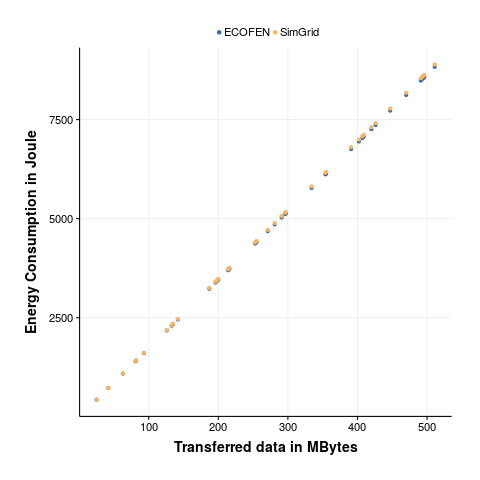
\includegraphics[width=0.47\linewidth]{images/ex11_energy_sg_vs_ns3}
		\label{fig:1l1f}
	}%
\centering
	\subfigure[1 Link 2 Flows]{
		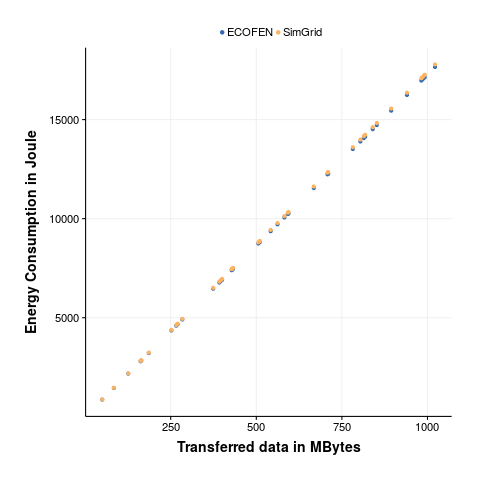
\includegraphics[width=0.47\linewidth]{images/ex12_energy_sg_vs_ns3}
		\label{fig:1l2f}
	}%
	
	\subfigure[1 Link 4 Flows]{
		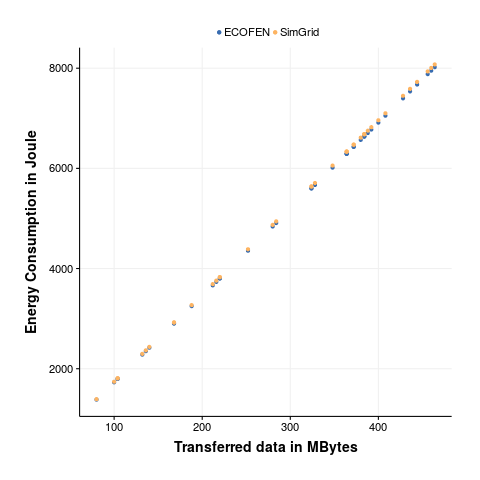
\includegraphics[width=0.47\linewidth]{images/ex10_energy_sg_vs_ns3}
		\label{fig:1l4f}
	}%
\centering
	\subfigure[3 Link 1 Flows]{
		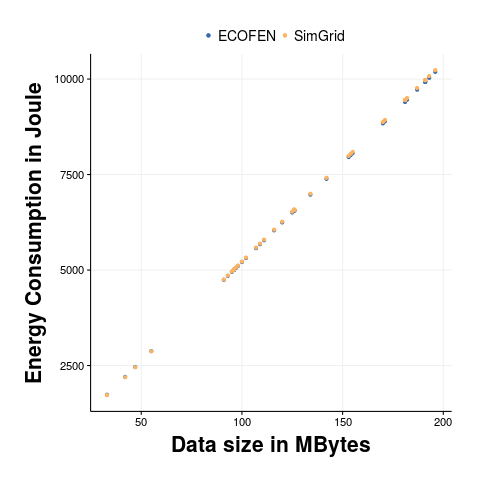
\includegraphics[width=0.47\linewidth]{images/ex13_energy_sg_vs_ns3}
		\label{fig:3l1f}
	}%

	\subfigure[3 Link 2 Flows]{
			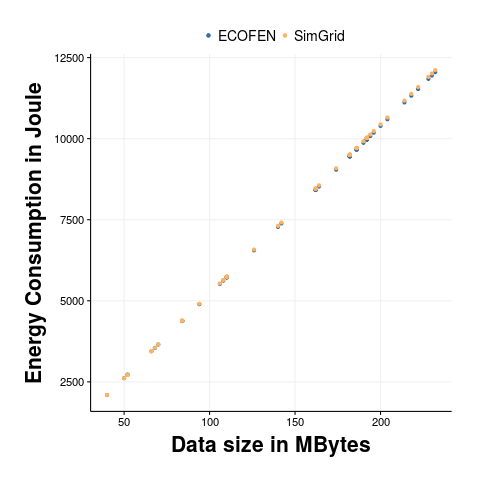
\includegraphics[width=0.47\linewidth]{images/ex15_energy_sg_vs_ns3}
			\label{fig:3l2f}
		}%
	\caption{Predicted energy consumption comparison of ECOFEN (blue dots) and SimGrid (orange dots) as a function of transferred Bytes for different path length and flow amount}
	\label{fig:sgvsns3scenario}
\end{figure}

\todo[inline]{You need to increase the font size of the figures below (legends and axis labels)}

\begin{table}
	\begin{tabular}{|>{\centering\arraybackslash}m{1.6cm}|>{\centering\arraybackslash}m{1.9cm}|>{\centering\arraybackslash}m{1.8cm}|>{\centering\arraybackslash}m{3.0cm}|>{\centering\arraybackslash}m{1.1cm}|>{\centering\arraybackslash}m{1.6cm}|} 
		\hline 
		\textbf{Scenario} &	\textbf{Mean of ECOFEN}&\textbf{Mean of SimGrid} & \textbf{CI  of Difference in mean} & \textbf{P-value}& \textbf{\% of Difference}\\ 
		\hline 
		1L1F&4837.2&4869.6&[-1156.3,1091.5]&0.9544&0.283\\
		\hline
		1L2F& 9672.6&9739.0& [-2314.2,2181.3]&0.9532&0.295\\ 
		\hline
		1L4F&5250.8&5286.9& [-720.10,647.90]&0.9169&0.297\\ 
		\hline	 
		3L1F&6804.9&6828.8& [-1024.9,977.1]&0.9622&0.124\\ 
		\hline
		3L2F&7896.6& 7931.9& [-1061.4,990.6]&0.9457&0.168\\ 
		\hline
	\end{tabular} 
	\caption{Unequal variance t-test statistics obtained using R. The confidence interval (CI) values in the fourth column are computed for the difference of the two energy consumption estimations and the last column values are obtained from mean log error as explained in \cite{DBLP:journals/tomacs/VelhoSCL13}}
	\label{table:welchtest}
\end{table}
 
\todo[inline]{You have to comment these results (you cannot assume people will read the figures and tables). So you have to say for instance that in the best/worst case we have an error of X, which is really good...}

 
\section{Scalability Validation}
For validating the scalability of the implemented flow-level model, we run also two sets of experiments. In the first set, our goal is to investigate the scalability of the model when the path length increases. For these experiments we use path length values of 1, 2, 4, 6, 8 and 10. We fix the number of flows at 2 and the data size at 200 MB. In the second set, we examine the scalability as the data size increases. In this case, we keep the path length at 1 and the number of flows at 2, but we vary the data size randomly between 50 and 550 MB. The total number of data size values within this range was 21. 

Both of these experiments were carried out using the Grid'5000 testbed, supported by a scientific interest group hosted by Inria and including CNRS, RENATER and several Universities as well as other organizations\footnote{https://www.grid5000.fr/mediawiki/index.php/Grid5000:UsagePolicy}. The machine we used is SUN FIRE X2270 which have Intel Xeon X5570 2.93 GHz 2 CPUs, 4 cores per CPU and 24 GB RAM running Debian version 8 (jessie) operating system.

For each set of experiments, we use the Debian command, /usr/bin/time, to collect simulation run time and peak memory usage data. We run each experiment within each set seven times i.e., 7 run for each link in the first set and 7 run for each data size in the second set. Figure~\ref{fig:scallinks} shows the runtime and memory usage comparison as the path length increases. Figure~\ref{fig:scaldata}, on the other hand, shows the runtime and peak memory usage comparison as the data size increases.

\begin{figure}[ht]
	\centering
	\subfigure[Runtime]{
		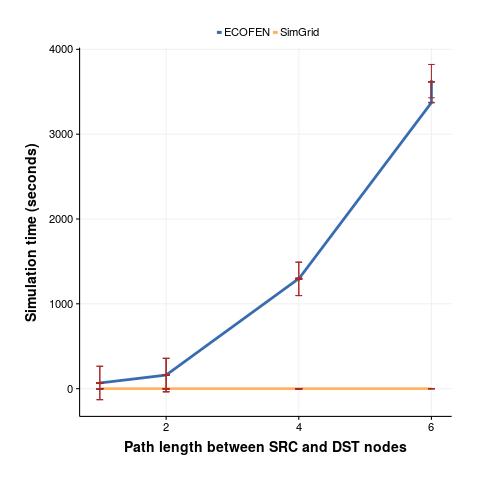
\includegraphics[width=0.5\linewidth]{images/ex16_linksize_sg_vs_ns3}
		\label{fig:lnkruntime}
	}%
	\centering
	\subfigure[Peak Memory Usage]{
		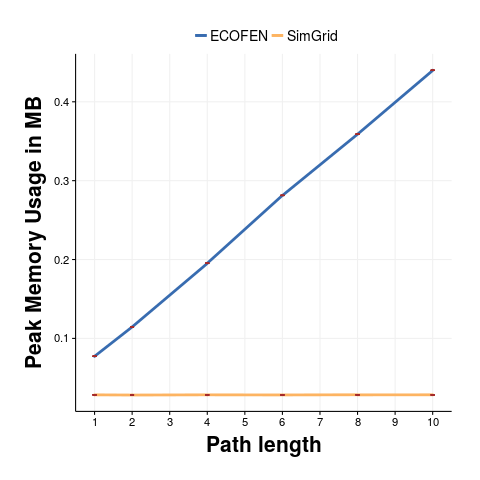
\includegraphics[width=0.5\linewidth]{images/ex16_linksizeM_sg_vs_ns3}
		\label{fig:lnkmem}
	}%
	\caption{Run time and peak memory usage comparison of ECOFEN and the flow-level model as the path length increases. In the figure the confidence interval for each experiment is also shown as a bar}
	\label{fig:scallinks}
\end{figure}

\begin{figure}[ht]
	\centering
	\subfigure[Runtime]{
		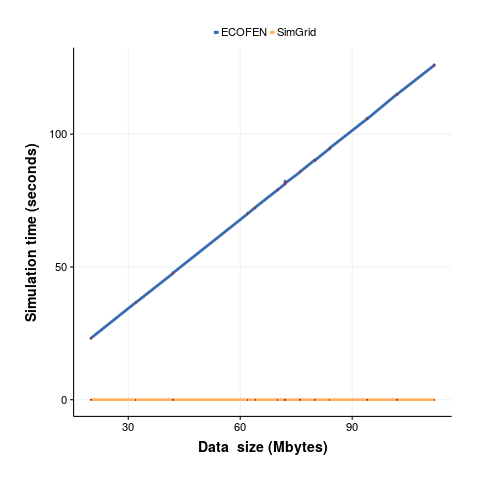
\includegraphics[width=0.47\linewidth]{images/ex21_datasize_sg_vs_ns3}
		\label{fig:datruntime}
	}%
	\centering
	\subfigure[Peak Memory Usage]{
		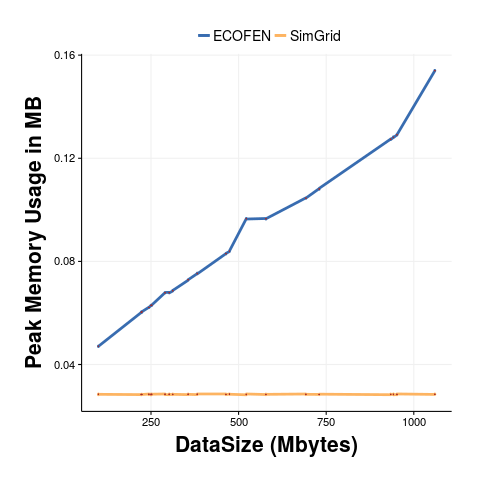
\includegraphics[width=0.47\linewidth]{images/ex21_DataSizeM_sg_vs_ns3}
		\label{fig:datmem}
	}%
	\caption{Run time and peak memory comparison of ECOFEN and the flow-level model as the data size increases. In the figure the confidence interval for each experiment is also shown as a bar}
	\label{fig:scaldata}
\end{figure}

\todo[inline]{You need to increase the font size of the figures below (legends and axis labels)}

\begin{table}
	\begin{tabular}{|>{\centering\arraybackslash}m{1.1cm}|>{\centering\arraybackslash}m{1.1cm}|>{\centering\arraybackslash}m{1.8cm}|>{\centering\arraybackslash}m{2.0cm}|>{\centering\arraybackslash}m{2.0cm}|>{\centering\arraybackslash}m{3.1cm}|} 
		\hline 
		\textbf{Link} &	\textbf{Flow}&\textbf{Data size} & \textbf{Average seconds SimGrid} & \textbf{Average seconds Ecofen}& \textbf{Runtime efficiency of Simgrid}\\ 
		\hline 
		1&2&100&0.3&132.95&443 times\\
		\hline
		10&2&100&0.3&817.02&2723 times\\ 
		\hline
		1&2&111&0.3&74.14&243 times \\ 
		\hline	 
		1&2&530&0.3&351.62&1172 times\\ 
		\hline
	\end{tabular} 
	\caption{Simulation time (runtime) comparison of SimGrid and ECOFEN. The first and the second rows compare at minimum and maximum path length values whereas the third and fourth column compare at minimum and maximum data size values. At each row the data size value has to be multiplied by the flow number to get the total data size}
	\label{table:runtime}
\end{table}

\begin{table}
	\begin{tabular}{|>{\centering\arraybackslash}m{1.1cm}|>{\centering\arraybackslash}m{1.1cm}|>{\centering\arraybackslash}m{1.8cm}|>{\centering\arraybackslash}m{2.0cm}|>{\centering\arraybackslash}m{2.0cm}|>{\centering\arraybackslash}m{3.1cm}|} 
		\hline 
		\textbf{Link} &	\textbf{Flow}&\textbf{Data size} & \textbf{Average memory SimGrid} & \textbf{Average memory Ecofen}& \textbf{Memory efficiency of Simgrid}\\ 
		\hline 
		1&2&100&0.028&0.077&2.7 times \\
		\hline
		10&2&100&0.028&0.44&15.5 times \\ 
		\hline
		1&2&111&0.028&0.06&2.12 times \\ 
		\hline	 
		1&2&530&0.028&0.15&5.4 times\\ 
		\hline
	\end{tabular} 
	\caption{Peak memory usage in mega Bytes (MB) comparison of SimGrid and ECOFEN. The first and the second rows compare at minimum and maximum path length values whereas the third and fourth column compare at minimum and maximum data size values. At each row the data size value has to be multiplied by the flow number to get the total data size}
	\label{table:peakmemory}
\end{table}

\todo[inline]{Here again, you have to comment the results. You can for instance write: this curves follows a proportional behavior and is provides simulation duration at least twice bigger than the other option... This clearly shows the validity/interest/suitability of our model for studying large-scale networks... (or things like this)}

From the accuracy and scalability experiments results presented in this chapter, we can clearly see that the implemented flow-level energy consumption model gives very good estimation prediction with relative error below 1\% and the runtime scalability is orders of magnitude faster than the packet-level counterpart. Table~\ref{table:runtime} shows that SimGrid is 2 to 3 orders of magnitude faster than ECOFEN and Table~\ref{table:peakmemory} shows SimGrid is 2 to 15 times more memory efficient. 


 
\chapter{Discussion}
\label{chapter:discussion}

In this research our objective was to investigate the level of accuracy and scalability obtained from flow-level models for estimating energy consumption of large-scale network. In order to achieve this goal we layout a research method that describes the steps that we followed from start to finish. 

Following our method, we started by studying literature to explore the state-of-the-art in the area of energy consumption of large-scale networks and the simulation frameworks available for estimating the consumption. From our literature study, we have learned that the energy consumption of a network equipment is characterized by two properties: idle power consumption and dynamic power consumption as a result of data transfer task. We have also learned that there are very few packet-level simulators proposed for estimating energy consumption of large-scale networks.

It is already known that packet-level simulators are more accurate in modeling a given network phenomenon compared to flow-level simulators but less scalable in terms of runtime and memory usage performance metrics~\cite{DBLP:conf/infocom/LiuFGKT01}. The accuracy of packet-level simulators comes from the detailed information they capture about simulated network phenomenon, they strive to capture packet-level details of the simulated network phenomenon. Flow-level simulators, on the other hand abstract away low-level details and model a given network phenomenon using analytical equations. Loosing low-level details allows flow-level models to scale well when the size of the simulated network increases. 

Due to this trade-off between level of details and scalability between the two simulation approaches, in our research, we stated the following hypothesis in order to investigate the level of accuracy and scalability we can get from flow-level models.

``\emph{flow-level energy consumption models can give reasonably accurate estimation and they can also be significantly more scalable than packet-level models}``

In order to test this hypothesis, we first implemented a flow-level energy consumption model that we found in literature for SimGrid and then conducted accuracy and scalability experiments as we have described in Chapter~\ref{chapter:evaluation}. 

The results of the accuracy validation experiments show that in fact very good energy consumption estimation accuracy can be obtained using flow-level models. For all the five scenarios run, the observed relative error lies approximately between  0.1\% and 0.3\% compared to the packet-level model used in ECOFEN. Our unequal variance t-test statistical test with p-value around 0.9 also tells that statistically the estimation difference between the packet-level simulator and the flow-level simulator is not significant. This confirms the first half of our hypothesis that flow-level models can give reasonably accurate estimations. The condition that should be satisfied in our model to let this hypothesis hold true is, correct time prediction, since our analytical equation (flow-level model) uses simulated time as one of its parameter. 

During our experimentation, we have noticed that there is significant difference between ECOFEN (or NS-3) and SimGrid on predicting the simulated time required to transfer a given amount of data. For a given data transfer, at a given latency value, SimGrid's predicted time continues to decrease as bandwidth increases whereas ECOFEN stops to decrease approximately when the bandwidth goes above 100 Mbps as shown in Figure~\ref{fig:bandwidthvstime}. Since addressing this problem is beyond the scope of our work, the approach we followed to avoid estimation error due to this time discrepancy is that we restricted all our experiments to bandwidth values where the two simulators closely agree on predicted time values.

Another point we like to point out about our accuracy validation experiments is that, there are additional tests that should be conducted to validate the correctness of the implemented model in different data transfer scenarios. For example SimGrid support simulating simultaneous TCP flows in same or different directions. All of the flows that we have used in our experiments were in the same direction. 

Concerning the scalability, the runtime and peak memory usage experiment results confirmed the second half of our hypothesis which states that flow-level models are significantly more scalable than their packet-level counter part. With the runtime performance metrics in Table~\ref{table:runtime}, we showed that SimGrid is 243 to 2723 times faster than ECOFEN. Similarly in Table~\ref{table:peakmemory} we have shown that SimGrid is 2 to 15 times more memory efficient than ECOFEN. Actually the scalability performance did not come directly from our implementation. It is due to the scalability of the underlying flow-level model of SimGrid. The scalability of SimGrid is already confirmed in other research works performed in the area of large-scale distributed systems~\cite{DBLP:conf/ccgrid/QuinsonRT12,DBLP:journals/jpdc/CasanovaGLQS14}.

Two of the limitations of our work is related to SimGrid's TCP model. The first one is that the TCP model in SimGrid can work in both half-duplex and full-duplex mode, however, our implementation works only in half-duplex mode. The second one  is that SimGrid uses different bandwidth sharing options that determine how the bandwidth is shared among the flows traversing a given link. In our implementation, we have only considered the option which shares bandwidth fairly among the flows. 

The other limitations of our work come from our scope. We have first limited our study to communicating components of large-scale networks. There are other energy consuming components such as data-center infrastructure facilities (which includes power provisioning, cooling and lighting components) that should be modeled in order to give full energy consumption estimation of a given large-scale network. Our work was also limited to the wired network components. As a result, we have not considered any communicating components that are involved solely on the wireless network, such as, Wi-Fi access points. 

Using our implementation together with already existing power consumption model of SimGrid for CPUs, it is possible to simulate energy consumption of computing and communicating components of large-scale networks. However, using present implementation, it is only possible to experiment on one kind of energy saving techniques: switching links ON/OFF. One can experiment on the effects of switching network components on or off to study the resulting energy cost difference. 

Other experiments, such as, investigating the effects of activating adaptive link rate energy saving mode on a link, can not be conducting using the current implementation. However, the current implementation can be extended to allow this feature by following the P-state approach implemented in the existing CPU energy consumption model. Similarly to CPU's P-state, a link can have multiple data transmission rate levels. 

We would like to recommend three areas for future researchers who would be willing to extend our work. First, to include in our model other features of SimGrid's TCP model such as full-duplex and different bandwidth sharing options.  Second, to consider other energy saving levers such as adaptive link rate. Third, to propose and implement flow-level energy consumption model for wireless network components following the method that we proposed in this manuscript. 

 
\chapter{Conclusions}
\label{chapter:conclusions}

In this thesis, we aimed at investigating the level of energy estimation accuracy and performance scalability that can be obtained from flow-level energy consumption models. In order to achieve this goal we outlined a research method and following this method we designed, implemented, and validated flow-level energy consumption models for SimGrid simulator. 

Using our validation experiments we have shown that the implemented flow-level model registered less than 1\% estimation error and it is also at least 2 times faster than the packet-level model. From these results we can conclude that given accurate simulated time prediction, our flow-level model gives very accurate energy consumption estimation and it is also significantly scalable. 

These findings suggest that, in general, even though flow-level models capture less detail about the reality they model, compared to packet-level models, the loss of detail might not result in significant loss of accuracy. 




% Load the bibliographic references
% ------------------------------------------------------------------
% You can use several .bib files:
% \bibliography{thesis_sources,ietf_sources}
\bibliography{sources}


% Appendices go here
% ------------------------------------------------------------------
% If you do not have appendices, comment out the following lines
\appendix
\chapter{First appendix}
\label{chapter:first-appendix}

This is the first appendix. You could put some test images or verbose data in an
appendix, if there is too much data to fit in the actual text nicely.

For now, the Aalto logo variants are shown in Figure~\ref{fig:aaltologo}.

\begin{figure}
\begin{center}
\subfigure[In English]{
\includegraphics[width=.8\textwidth]{images/aalto-logo-en}}
\subfigure[Suomeksi]{
\includegraphics[width=.8\textwidth]{images/aalto-logo-fi}}
\subfigure[P� svenska]{
\includegraphics[width=.8\textwidth]{images/aalto-logo-se}}
\caption{Aalto logo variants}
\label{fig:aaltologo}
\end{center}
\end{figure}


% End of document!
% ------------------------------------------------------------------
% The LastPage package automatically places a label on the last page.
% That works better than placing a label here manually, because the
% label might not go to the actual last page, if LaTeX needs to place
% floats (that is, figures, tables, and such) to the end of the 
% document.
\end{document}
